% 原文 p.243
\hypertarget{srcpage:243}{}\label{srcpage:243}
\sectionlink{バッキーボールとSQUID：デコヒーレンスの働きを観測する}
\setcounter{footnote}{0}
1990年代半ばまで、デコヒーレンスは主に理論模型を通じて研究されていた。第3章で述べたように、1985年にJoosとZeh\cite{ref007}は、塵の粒や大きな分子のような、極めて小さな物体の空間的重ね合わせ状態でさえ、ごくわずかな環境の散乱によって急速にデコヒーレンスすることを示した。また、Zurekが1984年に導いた、空間的デコヒーレンス率の概算式(2.113)\cite{ref012}は、巨視的尺度では、デコヒーレンスが散逸に比べて圧倒的に速いことを示唆した。これらの結果から、デコヒーレンスは極めて効率的かつ高速であるという一般的理解と、日常世界の非古典的重ね合わせは、どれも直ちにデコヒーレンスするという一般的予測が生まれた。

ここまでは、1980年代に知られていた。少なくとも、そうではないかと考えられていた。しかし、決定的に欠けていたのは、デコヒーレンスの作用により、重ね合わせ状態が徐々に観測できなくなる様子を示し、その動力学を実証する実験であった。経験世界に関係するあらゆる長さの尺度では、Schrödingerの猫状態の観測を阻むほど、デコヒーレンスは強く速い、と述べるだけでなく、そのような実験によって、この量子から古典への移行がどう起きるかを直接見られるはずである。デコヒーレンスの滑らかな作用が量子的特徴を運び去り、対象の物体を無事に古典領域へ送り込む様子を観測でき、さらに、その後量子コヒーレンスを回復させ、量子から古典への移行が本当に双方向の過程であることさえ示せるかもしれない。実験パラメーターを操作することで、この過程の動力学と性質を変え、基本的な量子・古典境界というCopenhagenの見方（8.1節参照）に挑むことができる。最後に、デコヒーレンスの理論模型を試し、実際の実験環境における環境相互作用の効果を、本当にどこまで捉えているかを調べることもできる。

そのような実験の有用性と面白さを、読者にも納得していただけたことを願いつつ、デコヒーレンスの実験を実現する際に、直ちに直面する困難を見よう。デコヒーレンスの漸進的な作用を観測するためには、何をする必要があるだろうか。第一に、非古典的重ね合わせ状態に系を準備できなければならない。もちろん、系はデコヒーレンスを十分に受けやすくするため、ある最低限の「大きさ」を持つべきである。単一の電子ではなく、できれば、
% 原文 p.244
\hypertarget{srcpage:244}{}\label{srcpage:244}
数個のもつれた光子や分子のような、中間的尺度の系が望ましい。しかし、ここに落とし穴がある。そのような系の重ね合わせ状態は通常、実験で分解できるよりもはるかに速くデコヒーレンスすることを、理論研究から知っている。したがって、デコヒーレンスが速過ぎず、しかも十分によく制御できるよう、非常に巧妙に実験を設計しなければならない。さらに、重ね合わせ状態を作ったら、あまり余分なデコヒーレンスを加えずに、系の状態を連続的に監視する手段も必要になる。これらの望ましい性質をすべて考えると、デコヒーレンス実験の実現は、非常に特殊な系と観測技術を必要とする、手ごわい課題である。

本章では、実験室で「Schrödingerの子猫」を作り、デコヒーレンスによって実効的に古典的な系へ変わる様子を、理論的予測との印象的な一致の下で観測できるようにした、近年の実験をいくつか述べる。6.1節では、漸進的なデコヒーレンス過程の観測を初めて可能にした実験を論じる。これは、電磁場の異なる状態の重ね合わせに基づく実験であった。6.2節では、かなり重い$\mathrm C_{70}$分子について、干渉模様と、デコヒーレンスによるその消失が観測された実験を述べる。6.3節では、超伝導二準位系、すなわち「量子ビット」系の実験に焦点を当てる。最後の6.4節では、将来のデコヒーレンス研究の有望な候補である、Bose--Einstein凝縮と量子電気機械系という、ほかの二つの実験領域を概説する。

\subsectionlink{最初の画期的成果：共振器中の原子}
1996年には、中間的尺度のSchrödingerの猫状態の生成と検証について、いくつもの実験的突破があった。これらの実験の基本機構は、Schrödingerが猫の逆説で最初に考えたもの（第1章参照）と似た過程に根ざし、von Neumannの測定図式（2.5.1節参照）で形式的に記述できる。比較的容易に重ね合わせ状態$(|s_1\rangle+|s_2\rangle)/\sqrt2$へ準備できる微視的な系Sを、中間的尺度または巨視的な装置Aと相互作用させ、後者が$\{|s_1\rangle,|s_2\rangle\}$基底でSの状態を「測定」するようにする。ここで測定とは、量子相関を形成するという、一般的なvon Neumannの意味である（2.5.1節参照）。これによって、もつれた結合状態が得られる［(2.54)と比較］。
\begin{equation}
|\Psi\rangle=\frac1{\sqrt2}(|s_1\rangle|a_1\rangle+|s_2\rangle|a_2\rangle).\tag{6.1}
\end{equation}
したがって、中間的尺度または巨視的な結合系SAは、今や重ね合わせ、すなわち「猫」状態$|\Psi\rangle$で記述される。

Monroeたち\cite{ref246}は、この原理を使い、捕獲した単一の${}^9\mathrm{Be}^+$イオンについて、中間的尺度の距離だけ離れた、空間的によく局在した二つのコヒーレント状態波束の重ね合わせを作った。
% 原文 p.245
\hypertarget{srcpage:245}{}\label{srcpage:245}
各波束は、イオンの異なる微視的な内部電子状態と相関していた。したがって、イオンは(6.1)の形の、もつれた猫状態、すなわち
\begin{equation}
|\Psi\rangle=\frac1{\sqrt2}(|x_1\rangle|\uparrow\rangle+|x_2\rangle|\downarrow\rangle)\tag{6.2}
\end{equation}
で記述される。ここで$|x_i\rangle$は$x_i$付近に局在した二つの波束、$|\uparrow\rangle$と$|\downarrow\rangle$は関係する二つの電子状態を表す。Monroeらは、超微細基底状態の対を用いた。先に導入した記法では、これらの電子状態が系Sに対応し、波束の二つの異なる空間領域が、中間的尺度の「計器」Aとして働く。

実験では、波束の中心は約80nm離れており、各波束の幅約7nmよりはるかに大きかった。重ね合わせの存在は、干渉模様を明示的に観測することで検証された。Monroeらは、実験でデコヒーレンスを調べるための技術をいくつか指摘したが、この問題を実際に実験的に調べたわけではなかった。

この野心的な目標は、同年、ParisのEcole Normale SupérieureのMichel Bruneたちによる、注目すべき実験\cite{ref247}で達成された（この実験の分かりやすい総説は\cite{ref248}も参照）。研究者たちは、物質粒子の重ね合わせの代わりに、古典的に区別できる位相を持つ放射場の、中間的尺度の猫状態を作り、その重ね合わせがデコヒーレンスによって徐々に壊れる様子を「見た」。この実験では、微視的な系Sと「計器」Aが、物理的に別々の系として実現されるため、Monroeらの実験よりも、元のSchrödingerの猫の設定の精神にさらに近い。

実験の基本的な考えは、次のとおりである。原子を、二つのエネルギー固有状態$|g\rangle$と$|e\rangle$の重ね合わせに準備し、電磁場のコヒーレント状態$|\alpha\rangle$を含む共振器を通過させる。場は、原子が$|e\rangle$状態なら、そのコヒーレント状態が位相シフト$\varphi$を受けて、$|\alpha\rangle\to|e^{i\varphi}\alpha\rangle$となり、原子が$|g\rangle$状態なら何も起きないという仕方で、原子の状態を実効的に測定する。時間発展の線形性により、原子の重ね合わせが、結合した原子・場状態に刻み込まれる。
\begin{equation}
\frac1{\sqrt2}(|g\rangle+|e\rangle)|\alpha\rangle
\longrightarrow\frac1{\sqrt2}(|g\rangle|\alpha\rangle+|e\rangle|\alpha e^{i\varphi}\rangle).\tag{6.3}
\end{equation}
実験では、コヒーレント状態は約10個の光子からなり、達成される位相シフト$\varphi$は$\pi$程度なので、場の相対状態$|\alpha\rangle$と$|e^{i\varphi}\alpha\rangle$は、中間的尺度で異なる。したがって、(6.3)の右辺は、真に中間的尺度の猫状態を表す。後述する巧妙な方法で、重ね合わせ状態の存在を検証し、その漸進的なデコヒーレンスを観測する。以下、この実験をより詳しく説明する。

% 原文 p.246
\hypertarget{srcpage:246}{}\label{srcpage:246}
\subsubsectionlink{原子と場の相互作用およびRabi振動}
実験では、重ね合わせの「種」として働く微視的な系Sは、二つの円形Rydberg状態に対応する、異なる二つのエネルギー固有状態$|g\rangle$、$|e\rangle$の重ね合わせに準備した、Rb原子で実現される。これらは、大きな量子数$n$と、量子化軸方向の最大の軌道角運動量、すなわち$|m|=n-1$を持つ状態である。Bruneら\cite{ref247}は$n=50$と51を用いた。対応する価電子の確率密度はトーラス形で、価電子は量子化軸に垂直な平面内の、準古典的な円軌道を運動する。このような状態には、多くの興味深い性質がある。この実験で最も重要なのは、大きな磁気双極子モーメントのため、弱いマイクロ波放射とも強く相互作用することである。また、電子は原子核から遠く、したがって加速度が比較的小さいため、放射減衰時間が長い。これら二つの特徴により、デコヒーレンスの漸進的作用の観測に必要な、長寿命の原子・場相関を準備できる。

原子と外部振動場の相互作用が実験の主要要素なので、いわゆるRabi振動を簡単に復習しよう。原子の二つのエネルギー準位$|g\rangle$（エネルギー$E_g$）と$|e\rangle$（エネルギー$E_e$）だけが関係すると仮定できるとする。実験で用いる円形Rydberg準位は放射と非常に強く相互作用するので、これはよい近似である。このとき原子状態は、
\begin{equation}
|\psi_{\mathrm{atom}}\rangle=c_g(t)|g\rangle+c_e(t)|e\rangle\tag{6.4}
\end{equation}
と書ける。$c_g(t)$と$c_e(t)$は、$|c_g(t)|^2+|c_e(t)|^2=1$を満たす任意の複素係数である。場がない場合、原子のHamiltonianは、
\begin{equation}
\hat H_0=E_g|g\rangle\langle g|+E_e|e\rangle\langle e|.\tag{6.5}
\end{equation}
それでは、周波数$\omega$の外部正弦振動場を加えよう。この場は古典的に扱うが、それは次の理由によって、この実験では完全に正当な近似となる。実験に使われる、場を含む特定の共振器は非常に散逸的であり、環境と強く相互作用する。したがって場のエネルギーとコヒーレンスが絶えず共振器から漏れ出し、場を実効的に古典的にする。これもまたデコヒーレンス過程である\cite{ref249}。これは、実験の共振器内の平均光子数が1程度であり、量子的取扱いが必要に思えるにもかかわらず成り立つ。

場を加えると、原子のHamiltonianは、$\hbar\equiv1$として、
\begin{equation}
\hat H=\hat H_0+\frac\epsilon2e^{i\omega t}|g\rangle\langle e|+\frac\epsilon2e^{-i\omega t}|e\rangle\langle g|\tag{6.6}
\end{equation}
となる。Rabi周波数$\epsilon$は、原子と場の結合の尺度である。したがって、外場は原子準位$|g\rangle$と$|e\rangle$の間に遷移を誘起できる。
% 原文 p.247
\hypertarget{srcpage:247}{}\label{srcpage:247}
原子が初めに基底状態$|g\rangle$、すなわち$c_g(0)=1$、$c_e(0)=0$にあるとすると、簡単な計算から、時間$t$後に原子が$|e\rangle$状態に見いだされる確率が得られる。
\begin{equation}
|c_e(t)|^2=\frac{\epsilon^2}{\Omega^2}\sin^2\frac{\Omega t}{2}.\tag{6.7}
\end{equation}
ここで$\Omega\equiv\sqrt{\Delta^2+\epsilon^2}$は一般化Rabi周波数と呼ばれ、$\Delta=\omega-\omega_{eg}$は、場の周波数$\omega$と原子遷移周波数$\omega_{eg}\equiv E_e-E_g$との離調を表す。離調$\Delta$が大きいほど、状態$|\psi_{\mathrm{atom}}\rangle$の成分$|e\rangle$の最大振幅は小さくなることが分かる。

共鳴時、すなわち場の周波数$\omega$を原子遷移周波数$\omega_{eg}$へ調整し、$\Delta=0$とすると、$\Omega=\epsilon$である。このとき(6.7)は、
\begin{equation}
|c_e(t)|^2=\sin^2\frac{\epsilon t}{2}=\frac12(1-\cos\epsilon t)\tag{6.8}
\end{equation}
となる。すなわち、原子は二つのエネルギー準位$|g\rangle$、$|e\rangle$の間を、Rabi周波数$\epsilon$で往復する。特に、原子を$|g\rangle$または$|e\rangle$状態から出発させ、時間$\tau=\pi/(2\epsilon)$だけ場を加えると、いわゆる「共鳴$\pi/2$パルス」であるが、$|c_e(\tau)|^2=1/2$となり、原子の結果の状態は、等しい重みの重ね合わせ
\begin{equation}
|\psi_{\mathrm{atom}}\rangle\propto|g\rangle+e^{i\Phi}|e\rangle\tag{6.9}
\end{equation}
となる。$\Phi$は、ある実数の位相である。実験でRb原子の初期重ね合わせ状態を作る方法は、まさにこれである。

2.2.2節で概説したRamsey干渉法も、二つの$\pi/2$ Rabiパルスの適用に直接基づくことを指摘しよう。最初の$\pi/2$パルスは、(2.4)、(6.9)のように、二つの基底状態の重ね合わせを作る。一方、ある遅延時間後に加える二番目の$\pi/2$パルスは、展開係数の大きさが遅延時間の関数として変動する、最終状態(2.6)をもたらす。

\subsubsectionlink{猫状態を作る}
放射場の重ね合わせ状態は、実験で厳密にどのように作られるのだろうか。以下の議論では、各段階の模式的概観を示す図6.1を参照されたい。まず、図6.2に描いた実験配置を見よう。源Oから放出され、初期状態$|e\rangle$に準備されたRb原子は、$R_1$、C、$R_2$と名づけられた、三つの共振器を順に通過する。最初の共振器$R_1$の目的は、上述の方法でRb原子の重ね合わせ状態を作ることである。すなわち、原子遷移$|g\rangle\leftrightarrow|e\rangle$の周波数に等しい周波数の$\pi/2$パルスを原子へ加え、$\Phi=0$とした状態(6.9)、すなわち
% 原文 p.248
\hypertarget{srcpage:248}{}\label{srcpage:248}
\begin{figure}[htbp]\centering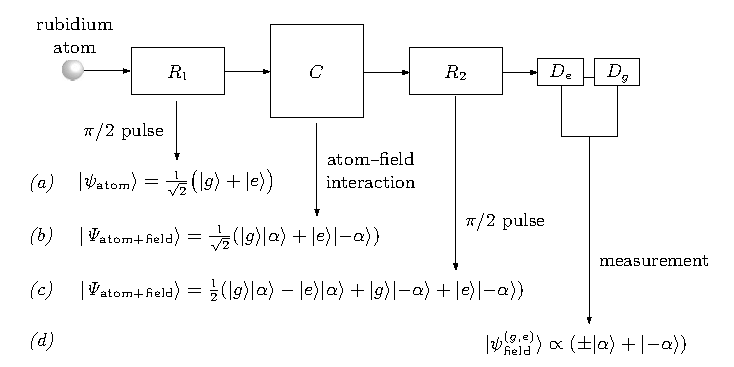
\includegraphics[width=.96\linewidth]{figures/ch06_fig01.pdf}
\caption{猫状態を生成する事象の系列。(a)共振器$R_1$で$\pi/2$パルスを加え、Rb原子を$|g\rangle$と$|e\rangle$の重ね合わせ(6.10)に準備する。(b)コヒーレント場$|\alpha\rangle$を含む共振器Cを通過するとき、原子が$|e\rangle$状態なら、場へ分散的位相シフト$|\alpha\rangle\to|-\alpha\rangle$を与える。原子は$|g\rangle$と$|e\rangle$の重ね合わせなので、もつれた原子・場状態［(6.15)参照］が作られる。(c)共振器$R_2$で、別の$\pi/2$パルスを原子へ加え、原子・場状態(6.17)へ導く。(d)検出器対$D_e$、$D_g$で原子のエネルギー状態$|g\rangle$または$|e\rangle$を測定し、共振器Cの状態を、もつれていない猫状態$|\Psi_{\mathrm{field}}^{(g,e)}\rangle\propto(\pm|\alpha\rangle+|-\alpha\rangle)$へ射影する。}
\end{figure}
\begin{figure}[htbp]\centering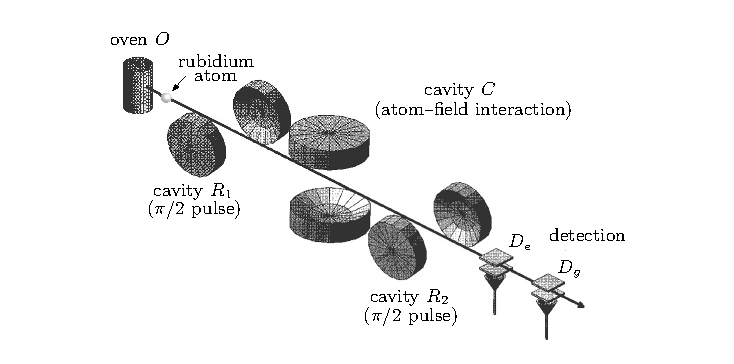
\includegraphics[width=.9\linewidth]{figures/ch06_fig02.pdf}
\caption{放射場の中間的尺度のSchrödingerの猫状態を作り、その漸進的デコヒーレンスを監視するために、Bruneら\cite{ref247}が用いた実験配置。炉Oから放出されたRb原子は、光子場を含む共振器$R_1$、C、$R_2$を順に通過し、電離箱$D_e$、$D_g$で検出される。許可を得て\cite{ref250}の図を改作。Copyright 1996 by the American Physical Society.}
\end{figure}

% 原文 p.249
\hypertarget{srcpage:249}{}\label{srcpage:249}
\begin{equation}
|\psi_{\mathrm{atom}}\rangle=\frac1{\sqrt2}(|g\rangle+|e\rangle)\tag{6.10}
\end{equation}
を作る。初期原子状態が$|g\rangle$なら、最終状態は$|\psi_{\mathrm{atom}}\rangle=(|g\rangle-|e\rangle)/\sqrt2$であっただろう。次に原子は共振器Cへ入る。共振器中の熱放射を最小にするため、Cは絶対零度近くの超伝導領域まで冷却される。共振器$R_1$とは対照的に、Cはいわゆる「Q値」が非常に大きい。Qは``quality''を表す。これは散逸損失が最小限となり、共振器内の光子寿命がかなり長いことを意味する。共振器は、約3cm離れた二枚の平行な鏡からなる。ただし鏡の間隔は調節でき、その結果、共振器内の放射の周波数を変えられる。この放射は、数個の光子を含むコヒーレント場からなる。

共振器の周波数が、準位$|g\rangle$からのいかなる遷移の共鳴周波数からも大きく外れているため、場と相互作用する$|g\rangle$状態には何も起こらない一方、別の準位$|i\rangle$、すなわち$n=52$の円形Rydberg状態を含む、$|e\rangle$からの遷移の周波数には、かなり近いことに注意することが非常に重要である。しかし、原子軌道に沿う場の強度の増減は非常にゆっくりなので、原子と場の相互作用はほぼ断熱的である。つまり、原子と場の間でエネルギー量子は交換されず、状態(6.4)の成分$|e\rangle$の振幅$|c_e(t)|$にも実際の変化は起きない。代わりに起こることが、非常に興味深い。共振器Cへ入った原子は、場に対する屈折媒質として働き、場の周波数にシフト$\delta\omega$を生じさせる。このシフトが有意になるのは原子が$|e\rangle$状態の場合だけで、$|g\rangle$状態では無視できることが分かる。原子と場の相互作用時間$\tau$を微調整することで、実験では、原子が$|e\rangle$状態の場合に、場に$\pi$に近い値の位相シフト$\varphi=\tau\delta\omega$を与える。

各光子へそのような位相シフト$\varphi$を加えると、コヒーレント状態$|\alpha\rangle$はどうなるだろうか。複素振幅$\alpha$の光子場のコヒーレント状態は、光子数固有状態$|n\rangle$の重ね合わせで定義される\cite{ref238,ref239,ref240,ref241}。
\begin{equation}|\alpha\rangle=\sum_{n=0}^\infty c_n|n\rangle,\tag{6.11}\end{equation}
ここで、
\begin{equation}c_n=e^{-|\alpha|^2/2}\frac{\alpha^n}{\sqrt{n!}}.\tag{6.12}\end{equation}
したがって光子数状態の分布は、平均光子数$\bar n=|\alpha|^2$のPoisson分布に従う。
\begin{equation}\wp(n)\equiv|c_n|^2=e^{-\bar n}\left(\frac{\bar n^n}{n!}\right).\tag{6.13}\end{equation}
各光子が位相シフト$\varphi$を受けると、状態$|\alpha\rangle$は、
% 原文 p.250
\hypertarget{srcpage:250}{}\label{srcpage:250}
\begin{equation}
|\alpha\rangle\longrightarrow e^{-|\alpha|^2/2}\sum_{n=0}^\infty e^{in\varphi}\frac{\alpha^n}{\sqrt{n!}}|n\rangle
=e^{-|\alpha|^2/2}\sum_{n=0}^\infty\frac{(e^{i\varphi}\alpha)^n}{\sqrt{n!}}|n\rangle=|e^{i\varphi}\alpha\rangle.\tag{6.14}
\end{equation}
となる。したがって、実験のように$\varphi=\pi$の位相シフトでは、コヒーレント場状態$|\alpha\rangle$は$|-\alpha\rangle$へ変換される。原子が共振器Cを通過した後、複合的な原子・場系は、状態［(6.3)参照］
\begin{equation}|\Psi_{\mathrm{atom+field}}\rangle=\frac1{\sqrt2}(|g\rangle|\alpha\rangle+|e\rangle|-\alpha\rangle)\tag{6.15}\end{equation}
で記述されることになる。図6.2の実験配置へ立ち戻ろう。実際には、$R_1$と同一の第三の共振器$R_2$が、原子軌道に沿って共振器Cの後にある。$R_2$内では、Cから出てきた原子へ、二回目の$\pi/2$パルスを加える。このパルスが、次の変換を実現することを思い出そう［(6.10)参照］。
\begin{equation}\begin{aligned}|g\rangle&\longrightarrow\frac1{\sqrt2}(|g\rangle-|e\rangle),\\|e\rangle&\longrightarrow\frac1{\sqrt2}(|g\rangle+|e\rangle).\end{aligned}\tag{6.16}\end{equation}
したがって、もつれた状態(6.15)は、
\begin{equation}\begin{aligned}
|\Psi_{\mathrm{atom+field}}\rangle&=\frac12(|g\rangle|\alpha\rangle-|e\rangle|\alpha\rangle+|g\rangle|-\alpha\rangle+|e\rangle|-\alpha\rangle)\\
&=\frac12(|\alpha\rangle+|-\alpha\rangle)|g\rangle+\frac12(-|\alpha\rangle+|-\alpha\rangle)|e\rangle.
\end{aligned}\tag{6.17}\end{equation}
となる。$R_2$の通過後、原子は二つの電離箱$D_e$、$D_g$へ入り、$|g\rangle$状態か$|e\rangle$状態かが測定される。状態(6.17)と量子力学の通常の射影公準によれば、測定後の場の状態は、原子が$|g\rangle$状態に見いだされるなら、
\begin{equation}|\psi_{\mathrm{field}}^{(g)}\rangle=\frac1{\mathcal N}(|\alpha\rangle+|-\alpha\rangle),\tag{6.18}\end{equation}
原子が$|e\rangle$状態に見いだされるなら、
\begin{equation}|\psi_{\mathrm{field}}^{(e)}\rangle=\frac1{\mathcal N}(-|\alpha\rangle+|-\alpha\rangle)\tag{6.19}\end{equation}
の、どちらかになる。ここで$\mathcal N$は規格化因子であり、$|\alpha|^2$が大きければ$\sqrt2$に非常に近い。簡単のため、以下では$\mathcal N=\sqrt2$と仮定しよう。

(6.18)、(6.19)から、今や異なる位相を持つ二つのコヒーレント場状態の重ね合わせを、実際に準備できたことが分かる。これらの状態の「猫らしさ」は、共振器C内の平均光子数$\bar n=|\alpha|^2$が増すほど大きくなる。
% 原文 p.251
\hypertarget{srcpage:251}{}\label{srcpage:251}
これらの重ね合わせ状態は、もつれた状態$|\Psi_{\mathrm{atom+field}}\rangle$［(6.15)参照］とは異なることに注意しよう。後者からは、場自体が重ね合わせにあるとはいえず、原子・場の結合系だけが重ね合わせで記述される。これに対して、共振器$R_2$を通過した後の原子状態の測定は、原子と場のもつれを解くので、(6.18)、(6.19)は放射場の真の重ね合わせ状態を表す。

重要な問いが一つ残る。重ね合わせ(6.18)、(6.19)を、対応する混合から、どう区別できるだろうか。これは、上述の方法で中間的尺度のSchrödingerの猫を作ることに成功したと主張するためだけでなく、私たちの主要目標、すなわちデコヒーレンスの作用を観測するためにも重要である。実験では、次節で説明する巧妙な仕掛けによって、この問題を解決する。
\subsubsectionlink{デコヒーレンスの漸進的作用を観測する}
最初の原子の通過と測定は、その状態に関する情報を共振器Cへ残すことに注意しよう。測定結果に応じて、C内の場の最終状態が、$|\psi_{\mathrm{field}}^{(g)}\rangle$または$|\psi_{\mathrm{field}}^{(e)}\rangle$となるからである。(6.18)、(6.19)から分かるように、この情報は、重ね合わせの成分$|\alpha\rangle$と$|-\alpha\rangle$の相対符号に符号化されている。デコヒーレンスは、このような位相情報を環境へ非局在化し、系の水準では利用できなくする傾向があることを知っている。その結果としてのコヒーレンスの減衰を、どう監視できるだろうか。

その仕掛けは、探針として働く第二の原子を、共振器列$R_1\to\mathrm C\to R_2$へ送ることである。第一の原子の通過後、十分速くこれを行えば、第一の原子についての情報は、共振器Cの場の状態へまだよく符号化されており、第二の原子はこの情報と相関する。注目すべき結果は、デコヒーレンスがなく、光子数が$\bar n=|\alpha|^2\gg1$なら、$D_e$または$D_g$での検出後、第二の原子は常に第一の原子と同じ状態に見いだされることである。

実際にそうなることは、次の簡単な計算から容易に分かる（図6.3参照）。原子1が$|e\rangle$状態で検出され、場の状態が$|\psi_{\mathrm{field}}^{(e)}\rangle$となったと仮定しよう。共振器$R_1$を通過した原子2は、重ね合わせ$|\psi_{\mathrm{atom2}}\rangle=(|g\rangle+|e\rangle)/\sqrt2$［(6.10)参照］で記述される。ここでは、基底状態$|g\rangle$と$|e\rangle$は原子2を指す。したがって、この原子と場の、初めの無相関な状態は、
\begin{equation}|\Psi_{\mathrm{atom2+field}}\rangle=\frac12(|g\rangle+|e\rangle)(-|\alpha\rangle+|-\alpha\rangle).\tag{6.20}\end{equation}
原子2が共振器Cを通ると何が起きるだろうか。原子が$|e\rangle$状態なら、場の状態は位相シフト$|\pm\alpha\rangle\to|\mp\alpha\rangle$を受けることを思い出そう。したがって、Cを通過した後の結合状態は、
% 原文 p.252
\hypertarget{srcpage:252}{}\label{srcpage:252}
\begin{equation}|\Psi_{\mathrm{atom2+field}}\rangle=\frac12(-|g\rangle|\alpha\rangle+|g\rangle|-\alpha\rangle-|e\rangle|-\alpha\rangle+|e\rangle|\alpha\rangle).\tag{6.21}\end{equation}
となる。次に原子は共振器$R_2$を通過し、$|g\rangle$と$|e\rangle$がこれらの状態の重ね合わせへ変換される［(6.16)参照］。したがって状態(6.21)は、
\begin{equation}\begin{aligned}
|\Psi_{\mathrm{atom2+field}}\rangle
&=\frac1{2\sqrt2}\bigl(-|g\rangle|\alpha\rangle+|e\rangle|\alpha\rangle+|g\rangle|-\alpha\rangle-|e\rangle|-\alpha\rangle\\
&\qquad-|e\rangle|-\alpha\rangle-|g\rangle|-\alpha\rangle+|e\rangle|\alpha\rangle+|g\rangle|\alpha\rangle\bigr)\\
&=\frac1{\sqrt2}|e\rangle(|\alpha\rangle-|-\alpha\rangle).
\end{aligned}\tag{6.22}\end{equation}
となる。$|\alpha\rangle$と$|-\alpha\rangle$が直交すると仮定すれば、共振器C内の光子数$\bar n=|\alpha|^2$が増すほどよい近似となるが、状態(6.22)に対応する原子2の縮約密度演算子は、
\begin{equation}
\hat\rho_{\mathrm{atom2}}=\operatorname{Tr}_{\mathrm{field}}|\Psi_{\mathrm{atom2+field}}\rangle\langle\Psi_{\mathrm{atom2+field}}|=|e_2\rangle\langle e_2|.\tag{6.23}
\end{equation}
直ちに、原子1が$|e\rangle$状態で検出されたとき、原子2を$|e\rangle$状態に見いだす確率$P_{ee}$は、$P_{ee}=1$となる。
% 原文 p.253
\hypertarget{srcpage:253}{}\label{srcpage:253}
原子1が$|g\rangle$状態で検出されたという仮定の下でも、同様の計算ができる。これで、二原子の完全な相関についての、上の主張が確立された。

\begin{figure}[htbp]\centering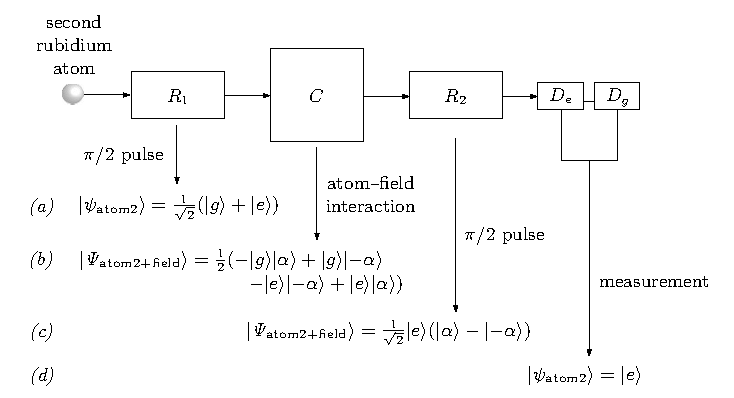
\includegraphics[width=.96\linewidth]{figures/ch06_fig03.pdf}
\caption{第一の原子が$|e\rangle$状態で検出されたと仮定したとき、共振器C内の場の重ね合わせ状態を検出し、そのデコヒーレンスを監視する事象の系列。(a)共振器$R_1$の$\pi/2$パルスが、第二のRb原子を$|g\rangle$、$|e\rangle$の重ね合わせ(6.20)に準備する。(b)原子は、第一の原子の通過後、重ね合わせ状態に残された共振器Cへ入る。原子2はC内の場へ別の位相シフトを与え、もつれた原子・場状態［(6.21)参照］を作る。(c)共振器$R_2$の$\pi/2$パルスが、場と原子のもつれを解く［(6.22)参照］。(d)場の状態$|\pm\alpha\rangle$が近似的に直交するなら、原子2は常に、原子1と同じ$|e\rangle$状態で検出される。したがって、二つの測定結果は完全に相関する。この相関の減衰は、共振器Cの猫状態のデコヒーレンスを意味する。}
\end{figure}

ゆえに、猫状態のデコヒーレンスを観測するために必要なのは、第一、第二の原子を送り出す時間間隔$T$を増やしながら、原子対の測定結果間の相関$P_{ee}(T)$、あるいは$P_{gg}(T)$の減衰を測定することだけである。$T$が場の重ね合わせの特徴的なデコヒーレンス時間よりはるかに小さければ、$P_{ee}(T)$は1に近くなる。重ね合わせがまだほとんどデコヒーレンスしていないときの、測定結果間の完全な相関を反映するのである。遅延時間$T$を長くすると、共振器内の重ね合わせは、ますますデコヒーレンスする。やがて、すべての相対位相情報、したがって第一の原子の状態の情報が環境へ非局在化し、場は非コヒーレントな統計的混合
\begin{equation}\hat\rho_{\mathrm{field}}=\frac12(|\alpha\rangle\langle\alpha|+|-\alpha\rangle\langle-\alpha|)\tag{6.24}\end{equation}
で記述される。このとき、第一、第二の原子の測定結果は完全に無相関となる。すなわち、第二の原子の測定結果はランダムであり、第一の原子の測定結果から独立になる。したがって、このデコヒーレンス過程は、$P_{ee}(T)$が$1/2$まで減衰することとして観測できる。

図6.4は、$P_{ee}(T)$の理論予測\cite{ref250}を示し、これは実験観測\cite{ref251}と非常によく一致した。$P_{ee}(T)$が初期値1からかなり急速に低下し、完全なデコヒーレンスに対応する$P_{ee}(T)=1/2$の平坦部に達する様子が明瞭に見える。読者は、$P_{ee}(T)$がある範囲の遅延時間$T$にわたり$1/2$付近にとどまった後、より大きい$T$で、なぜ突然また0へ向かって減衰するのかと、疑問に思うかもしれない。説明は非常に簡単である。共振器C内の光子寿命は有限なので、やがてC内に光子がなくなる。すると、Cを通過する原子に対する効果はなくなる。この場合、原子が受けるのは、共振器$R_1$と$R_2$の二つの$\pi/2$パルスだけであり、それらの合成効果は、初期状態$|e\rangle$を$|g\rangle$へ変換することである［(6.16)参照］。
\begin{equation}|e\rangle\xrightarrow{\pi/2}\frac1{\sqrt2}(|g\rangle+|e\rangle)\tag{6.25}\end{equation}
\begin{equation}\xrightarrow{\pi/2}\frac1{\sqrt2}\left[\frac1{\sqrt2}(|g\rangle-|e\rangle)+\frac1{\sqrt2}(|g\rangle+|e\rangle)\right]=|g\rangle.\tag{6.26}\end{equation}
したがって、原子は決して$|e\rangle$状態で検出されず、$T\to\infty$で$P_{ee}(T)\to0$となる。

図6.4のグラフから、場の重ね合わせの特徴的デコヒーレンス時間を読み取れる。実験では、それが二つの主要パラメーターに依存することが示された。
% 原文 p.254
\hypertarget{srcpage:254}{}\label{srcpage:254}
\begin{figure}[htbp]\centering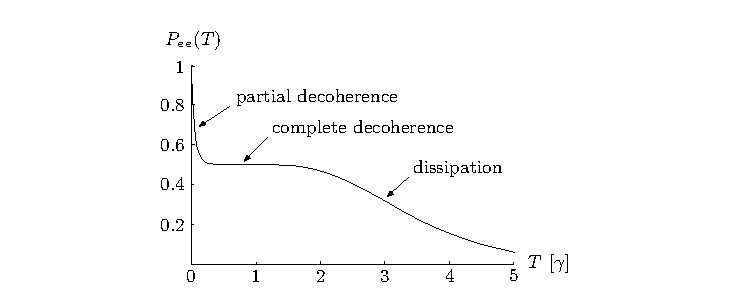
\includegraphics[width=.85\linewidth]{figures/ch06_fig04.pdf}
\caption{Davidovichら\cite{ref250}による、一対の原子が通過する遅延時間$T$への、同時確率$P_{ee}(T)$の依存性。初期の速い減衰は、共振器Cの猫状態のデコヒーレンスに対応し、$P_{ee}(T)=1/2$は完全なデコヒーレンスを表す。さらに大きな$T$では、共振器からの光子漏出によって$P_{ee}(T)$がさらに低下する。遅延時間$T$の単位は、共振器の特徴的散逸期間$\gamma$である。許可を得て\cite{ref250}の図を改作。Copyright 1996 by the American Physical Society.}
\end{figure}
\begin{enumerate}
\item 共振器Cを通過する$|e\rangle$状態の原子が、場へ誘起する位相シフト$\varphi$。$\varphi$が大きいほど、場の重ね合わせのデコヒーレンス時間が短いことが分かった。これはもっともである。重ね合わせ状態の「猫らしさ」は、各成分をどれほど識別できるかに依存する。$\varphi$が小さければ、場の状態$|\alpha\rangle$と$|e^{i\varphi}\alpha\rangle$［(6.14)参照］の重なりは大きい。他方、$\varphi$が最大値$\pi$へ近づくと、これは上の議論で仮定した値であり、実験で達成した位相シフトにも近いが、二状態は直交し、したがって最大限に区別される。
\item 共振器C内の平均光子数$\bar n=|\alpha|^2$。これも理にかなっている。光子が多いほど、状態$|\Psi_{\mathrm{field}}^{(g,e)}\rangle$［(6.18)参照］は、より中間的尺度のもの、最終的には巨視的なものとなり、したがって、より強くデコヒーレンスを受ける。また、与えられた位相シフト$\varphi$について、$\bar n$が大きいほど成分$|\alpha\rangle$と$|e^{i\varphi}\alpha\rangle$の重なりは小さくなり、より区別される。
\end{enumerate}
Bruneたちは実験でこれらのパラメーターを変え、デコヒーレンス率がそれに応じて変わる様子を観測した。注目すべきことに、結果はDavidovichら\cite{ref250}の理論予測と驚くほどよく一致した。中間的尺度の「Schrödingerの子猫」を生成し、存在を検証し、そのデコヒーレンスを制御された仕方で観測したのは、これが初めてであった。

% 原文 p.255
\hypertarget{srcpage:255}{}\label{srcpage:255}
Bruneたちが行った型の実験は、その後、さらに多くの実験を生み、上述の結果が確認され、拡張されてきた。たとえば、共振器CのQ値を改善する必要があるが、その光子数を増すことで、ますます大きな猫状態を作れる。最近の実験では、数十個の光子が使われている\cite{ref252}。この種の実験は一般に「共振器量子電気力学」、略して「共振器QED」と呼ばれる。Schrödingerの猫状態の生成と、そのデコヒーレンスの観測だけでなく、共振器QEDは、量子コンピューターの実現にも使える可能性がある。さらに学びたい読者には、Dutraの本\cite{ref253}が、よい、しかも楽しく読める入門となる。

\subsubsectionlink{Schrödingerの猫を生き返らせる}
デコヒーレンスが完全にユニタリーで、したがって原理的に可逆な過程であるにもかかわらず、私たちは量子から古典への移行を「一方通行」と考えがちである。量子コヒーレンスが失われると、物体は古典的に振る舞い、量子世界へ戻すものは何もないように見える。もちろん、2.7節のデコヒーレンスの一般的議論から、それがあらゆる実用的目的について不可逆とみなされる理由を知っている。系の水準へ重ね合わせを実際に「再局在化」する、すなわちデコヒーレンス過程を実効的に時間反転するには、環境を適切に制御しなければならず、それは通常、実際には不可能だからである。

2.13節では、完全に制御できるよう適切に設計した「人工的」環境と系を相互作用させることで、仮想的デコヒーレンスの一例である、真に可逆なデコヒーレンス過程を調べられることを指摘した。1997年、Bruneのグループ\cite{ref254}は、前の各節の共振器QED実験を修正し、そのような設計された環境を含める案を提案した。2007年現在、この提案はまだ実験的に実現されていない。主な理由は、二つの超伝導共振器の間の可逆的結合が必要で、それを実際に実現するのが難しいからである。それでも、実験の考え方は非常に興味深く、技術的障害が近い将来に克服される見込みも高いため、本節で提案を概説する。

実験配置は、基本的に前述のものと同じである（図6.2参照）。主要な違いは、超伝導共振器Cを、たとえば超伝導導波路を用いて、初め空の、第二の同一共振器$\mathrm C_2$へ線形結合することである。追加の$\mathrm C_2$と明瞭に区別するため、以下では最初の共振器Cを$\mathrm C_1$と呼ぶ。この結合によって、$\mathrm C_1$と$\mathrm C_2$はエネルギー、すなわち光子を交換できる。Rb原子が装置を通過し、その状態が$D_e$、$D_g$で測定された後、共振器$\mathrm C_1$は二つの場の状態$|\alpha\rangle$、$|-\alpha\rangle$の重ね合わせに残されること［(6.18)、(6.19)参照］、
% 原文 p.256
\hypertarget{srcpage:256}{}\label{srcpage:256}
そして、二成分の相対符号が、測定された原子状態の情報を符号化することを思い出そう。

二共振器の結合によって、この位相情報が「貯蔵庫」$\mathrm C_2$へ移ったとする。このとき$\mathrm C_1$の状態は、対応して混合(6.24)で記述されなければならない。提案の考え方は、$\mathrm C_1$と$\mathrm C_2$の結合が十分高い程度まで可逆なら、その後この情報伝達の向きを逆転し、$\mathrm C_1$の初期重ね合わせを回復するとともに、$\mathrm C_2$を初期の空の状態へ戻せる、というものである。こうして、$\mathrm C_2$が$\mathrm C_1$に対する制御可能な単一モード環境として働き、$\mathrm C_1$のSchrödingerの猫状態をデコヒーレンスさせ、その後再出現させる、可逆なデコヒーレンス過程を模擬できる。

この議論をもう少し精密にしよう。二共振器間で、エネルギーが周波数$\Omega_{\mathrm C}$で振動的に交換されるとする。この周波数は、$\mathrm C_1$の猫状態の準備時間が、エネルギー交換の一周期よりはるかに短くなるよう選ぶ。したがって、二共振器の結合は重ね合わせ状態の準備に影響しないと仮定する。結合は線形なので、$\mathrm C_1$のコヒーレント場$|\alpha(t)\rangle$は、$\mathrm C_2$に別のコヒーレント場$|\beta(t)\rangle$を生じさせる。$t=0$で$\mathrm C_2$が場を含まないことを考慮すると、$\alpha(t)=\alpha_0\cos(\Omega_{\mathrm C}t/2)$、$\beta(t)=\alpha_0\sin(\Omega_{\mathrm C}t/2)$と書ける。したがって、$\mathrm C_1$の初期猫状態［(6.18)、(6.19)参照］
\begin{equation}|\Psi_{\mathrm C_1}^{(g,e)}\rangle=\frac1{\mathcal N}(\pm|\alpha\rangle+|-\alpha\rangle)\tag{6.27}\end{equation}
は、結合系$\mathrm C_1+\mathrm C_2$のもつれた状態へ発展する。
\begin{equation}|\Psi_{\mathrm C_1+\mathrm C_2}^{(g,e)}\rangle=\frac1{\mathcal N}(\pm|\alpha(t)\rangle|\beta(t)\rangle+|-\alpha(t)\rangle|-\beta(t)\rangle).\tag{6.28}\end{equation}
その後の振る舞いは、二つのコヒーレント場状態$|\pm\alpha\rangle$の重なりが、平均光子数$\bar n=|\alpha|^2$が増すほど減少することから、容易に理解できる。時間$t=\pi/\Omega_{\mathrm C}$後には$\beta(t)=\alpha_0$となり、すべての光子が$\mathrm C_2$に集中する。したがって$|\pm\beta\rangle$は最大限に区別され、$|\pm\alpha\rangle$の識別可能性は最小になる。これは、重ね合わせ成分の相対符号についての情報を、$\mathrm C_1$の犠牲の下で、$\mathrm C_2$が最大限保持することを意味する。言い換えれば、$\mathrm C_1$だけへのどのような測定からも、相対符号について何も分からない。$\mathrm C_2$が位相情報を運び去り、$\mathrm C_1$は形式的に、$|\pm\alpha\rangle$の非コヒーレント混合(6.24)で記述される。

読者は、この状況が、環境に対応する状態が急速に直交し、系の密度行列で相対位相情報が減衰する、通常のデコヒーレンス過程の記述（2.7節参照）と、まさに類似していると気づくだろう。
% 原文 p.257
\hypertarget{srcpage:257}{}\label{srcpage:257}
ここでは$\mathrm C_2$が、まさに環境の役割を果たすため、この類似は予想どおりである。しかし、ここでの提案の決定的な違いは、特徴的時間$\tau=2\pi/\Omega_{\mathrm C}$、すなわち二共振器間のエネルギー交換周期後に、過程が完全に逆転することである。今や$|\pm\alpha\rangle$は、$t=0$と同じく再び最大限に区別される。相対符号についてのすべての情報を$\mathrm C_1$から取り出せ、$\mathrm C_2$の場の重ね合わせのコヒーレンスは回復している。

この漸進的デコヒーレンスと再コヒーレンスは、以前とまったく同じ方法、すなわち第二の原子を装置へ送り、二原子の通過の遅延時間$T$に対する同時確率$P_{ee}(T)$の依存性を測定することで観測できる。$\mathrm C_1$と$\mathrm C_2$の結合以外のデコヒーレンス源を無視すれば、$P_{ee}(T)$は、$n=1,2,\ldots$に対する時刻$T_n=n\tau=2n\pi/\Omega_{\mathrm C}$に、周期的に初期値1へ戻ると予想される。これらの時刻には、$\mathrm C_1$の猫状態のデコヒーレンスは完全に取り消されている。逆に、間隔$n\tau/2=n\pi/\Omega_{\mathrm C}$では、$\mathrm C_1$は非コヒーレント混合で記述され、原子1、2の測定結果は完全に無相関となり、$P_{ee}(n\tau/2)=1/2$となる。

この振る舞いを図6.5に示す。同時確率$P_{ee}(T)$を直接描く代わりに、Raimond、Brune、Haroche\cite{ref254}が最初に導入した、二原子相関関数$\eta(T)$を用いた。この関数は完全相関では$1/2$、完全なデコヒーレンスでは0となる。遅延時間が、特徴的時間$\tau=2\pi/\Omega_{\mathrm C}$の整数倍に等しいと、初期状態が回復し、コヒーレンスの復活が得られることが分かる。
\begin{figure}[htbp]\centering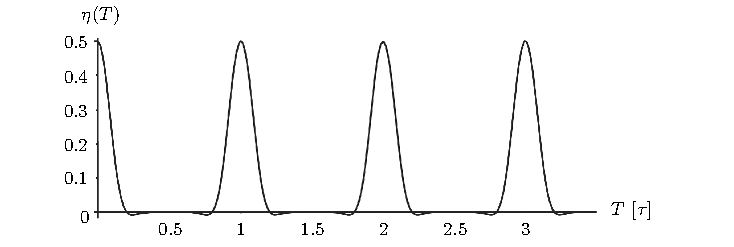
\includegraphics[width=.94\linewidth]{figures/ch06_fig05.pdf}
\caption{Raimond、Brune、Haroche\cite{ref254}が提案した再コヒーレンス実験における、遅延時間$T$に対する二原子相関関数$\eta(T)$の依存性。第二の共振器$\mathrm C_2$、すなわち貯蔵庫によって、$\mathrm C_1$からコヒーレンスが連続的に取り出され、戻される。これが$\mathrm C_1$の猫状態の周期的復活と、最大相関信号$\eta(T)=1/2$の再出現を生む。$T$の単位は、二共振器間でエネルギー、したがって位相情報を交換する特徴的周期$\tau=2\pi/\Omega_{\mathrm C}$である。$\mathrm C_1$の初期場は、平均5個の光子を含むとした。}
\end{figure}

% 原文 p.258
\hypertarget{srcpage:258}{}\label{srcpage:258}
もちろん、現実的な実験設定では、この復活過程は永遠には続かない。共振器$\mathrm C_1$と$\mathrm C_2$は、鏡面での光子損失のような、ほかのデコヒーレンス源や散逸効果を受けるからである。これらの過程は、図6.5の復活ピークの振幅を指数関数的に減衰させることが示されており\cite{ref255}、実際に数個以上のピークを観測できる見込みは低い。それでも、一つの復活ピークの観測だけでも、デコヒーレンスが少なくとも原理的には完全に可逆である事実を、印象的に実験で示すことになる。

\subsectionlink{$\mathrm C_{70}$分子による干渉実験}
本節では、University of ViennaのAnton Zeilingerのグループが行った、一連の実験を述べる。これらは本質的に、よく知られた二重スリット実験を高度に改良したものである。しかしここでは、光や電子のような微視的実体の代わりに、重い分子の干渉模様を観測する。これらの実験が注目すべきなのは、二つの理由による。第一に、通常なら明らかに「物質」の分類に入る物体の、量子的な「波動性」を示す。第二に、デコヒーレンスの連続的作用が、これらの物体から「量子性」を徐々に奪い、経験するおなじみの古典的物体へ変える様子を直接示す。詳しく述べる前に、先行する実験、すなわち単一電子で行われた二重スリット実験を、まず数段落で概説しよう。

\subsubsectionlink{電子による二重スリット実験}
2002年、Physics Worldの読者に、史上「最も美しい物理実験」を選ぶよう求めたところ、一位になったのは、単一電子による二重スリット実験\cite{ref256}だった。Feynmanは、二重スリット実験は「その中に量子力学の核心があり、実際、それは理論の唯一の謎を含む」現象であると述べたことで有名である\cite{ref257}。確かに、量子力学の奇妙な特徴を、これほど単純かつ完全に体現する、ほかの実験を想像するのは難しい。

興味深いことに、電子が二重スリットを通るという元の形でこの実験が実際に行われたのは、1961年、University of TübingenのGottfried Möllenstedtの学生、Claus Jönsson\cite{ref258,ref259}によってであった。Möllenstedtは、それ以前に、電子ビプリズムという別の装置、本質的には電子ビームを二分する非常に細い線を使い、電子の干渉を実験的に示していた。この方法は、19世紀初頭に英国の科学者Thomas Youngが、日光のビームを分け、光が波動的な強め合い・弱め合いの干渉効果を示すことを実証した実験\cite{ref260}で使った、紙片に似ている。
% 原文 p.259
\hypertarget{srcpage:259}{}\label{srcpage:259}
さらに意外かもしれないが、装置内に常に単一電子しかないことを保証した実験は、1989年になって初めて、HitachiのAkira Tonomuraたちが、Möllenstedtと同じく電子ビプリズムを用いて行った\cite{ref261}。得られた干渉模様を図6.6に示す。この実験は、干渉縞が電子間の相互作用で生じるのではなく、個々の電子の波動性によることを示し、量子力学の「謎」を明瞭に反映する。電子ビプリズム干渉計のデコヒーレンスは、最近SonnentagとHasselbach\cite{ref262}が調べた。彼らは、電子と、巨視的で散逸的な電子気体・フォノン気体環境とのCoulomb相互作用によって、干渉模様の可視度が減衰する様子を研究した。

\subsubsectionlink{実験配置}
重い分子の波動性を示すために、Zeilingerのグループが用いた実験配置を概説しよう。Markus Arndtたち\cite{ref263}が1999年のNature論文で報告した最初の実験では、その形から「バッキーボール」と呼ばれることの多い、$\mathrm C_{60}$分子が使われた（図6.7参照）。その後、Zeilingerのグループが2002年の論文\cite{ref264}で初めて結果を報告した実験は、さらに大きな、細長いバッキーボール形の$\mathrm C_{70}$分子と、異なる実験配置\cite{ref264,ref265,ref266,ref267}を用いて行われた。以下では、この後の一連の実験に基づいて論じる。

まず、$\mathrm C_{70}$分子が、電子などの微視的実体に比べて、どれほど重いかを実感しよう。
\begin{figure}[htbp]\centering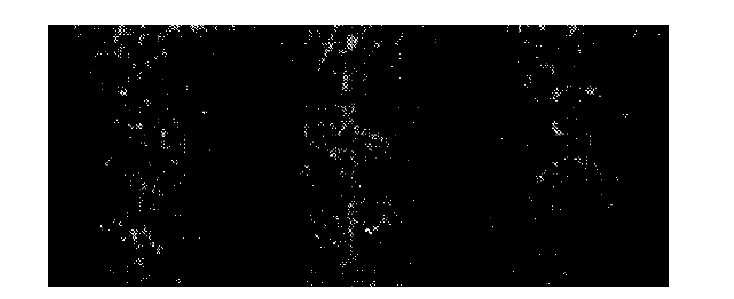
\includegraphics[width=.85\linewidth]{figures/ch06_fig06.pdf}
\caption{Tonomuraたち\cite{ref261}の二重スリット実験で得られた、単一電子の干渉模様。許可を得て\cite{ref261}から転載。Copyright 1989 American Institute of Physics.}
\end{figure}
% 原文 p.260
\hypertarget{srcpage:260}{}\label{srcpage:260}
各炭素原子は6個の陽子、6個の中性子、6個の電子を含むので、$\mathrm C_{70}$分子は合計1000個以上の微視的構成要素からなる。各分子は、高度に励起された内部回転・振動自由度を非常に多数持つ。このため、個々の分子に有限の温度を割り当てることができる。また、分子からの熱放射、すなわち光子の放出も観測できる\cite{ref267}。したがって、$\mathrm C_{70}$分子は、明らかに「粒子」の分類に入るように見える。
\begin{figure}[htbp]\centering
\includegraphics[width=.65\linewidth]{figures/ch06_fig07.pdf}
\caption{Arndtら\cite{ref263}の最初の物質波干渉実験で用いられた、$\mathrm C_{60}$分子の模式図。60個の炭素原子が、直径約1nmのバッキーボール形に並んでいる。}
\end{figure}

このような重い分子の干渉効果を観測するのは、なぜ難しいのだろうか。関係する量は、物質のde Broglie波長$\lambda=h/(mv)$であり、$m$、$v$はそれぞれ粒子の質量と速度である。したがって、粒子が重く速いほど、波長は短い。二重スリット型の実験で粒子の干渉を観測するには、スリット間隔、まして各スリットの幅が、波長程度でなければならない。実験の$\mathrm C_{70}$分子の典型的速度、約$100\,\mathrm{m/s}$では、de Broglie波長はわずか数pmである。このような狭いスリットを、これほど狭い間隔で作ることが不可能なのは、容易に想像できるだろう。

この困難をどう克服できるだろうか。Zeilingerのグループは、いわゆるTalbot--Lau効果に基づく、巧みな仕掛けで解決する。その基本原理は次のとおりである（図6.8参照）。平面波$f(z)=e^{2\pi iz/\lambda}$が、$+z$方向に進むとする。この入射波に直角に、平行なスリットの列からなる格子を置く。隣り合うスリットの間隔を$d$とする。このとき、格子の後方の距離
\begin{equation}L_\lambda=\frac{d^2}{\lambda}\tag{6.29}\end{equation}
の整数倍のところで、波の形が実際に格子模様と等しくなることを示せる。ここでは導かないが、短い導出は\cite{ref268}を参照されたい。言い換えれば、格子の後方$nL_\lambda$、$n=1,2,\ldots$の距離にスクリーンを置き、光で実験すると、
% 原文 p.261
\hypertarget{srcpage:261}{}\label{srcpage:261}
間隔$d$の明暗の帯が現れ、格子自体の像を作る。このTalbot--Lau効果は、真の干渉現象である。したがって、物質粒子で同じ実験を行い、「Talbot長」$L_\lambda$の整数倍のところに、格子模様と等しい密度模様を観測すれば、粒子の波動性を示したことになる。ただし、原理的には、格子が単に光線を遮る、いわゆるMoiré効果でも縞が生じる。しかしMoiré模様は波長$\lambda$に依存しない。ゆえに、本当にTalbot--Lau効果かを確かめるには、$\lambda$を変えながら模様の変化を観測すればよい。物質波の場合、$\lambda=h/(mv)$なので、粒子の平均速度$v$を変えることで実現する。
\begin{figure}[htbp]\centering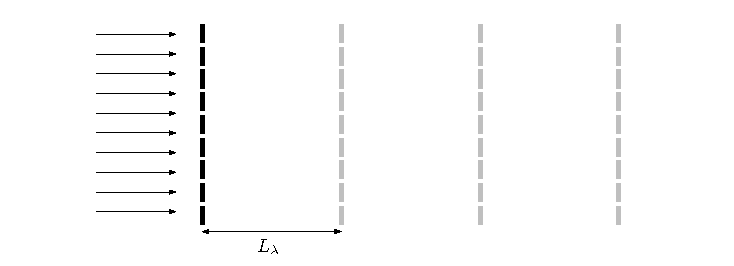
\includegraphics[width=.85\linewidth]{figures/ch06_fig08.pdf}
\caption{Talbot--Lau効果。左の格子を通る平面波は、格子から距離$nL_\lambda$、$n=1,2,\ldots$のところに、格子の像を作る。}
\end{figure}

簡単な評価から、$\mathrm C_{70}$分子の干渉効果を検出するTalbot--Lau法の利点を、直ちに納得できる。Zeilingerのグループの実験では、格子間隔$d$は約$1\,\mu\mathrm m$、分子波長は数pmである。したがって$L_\lambda\sim(10^{-6}\,\mathrm m)^2/(10^{-12}\,\mathrm m)=1\,\mathrm m$となり、干渉模様を観測するには、格子の後方の巨視的距離$L_\lambda$に、「スクリーン」、すなわち粒子検出器を置くだけでよい。実際の実験距離は$L_\lambda=38\,\mathrm{cm}$である。そこで分子速度を変えたとき、特徴的な波長依存性を示す、周期$d$の粒子密度変化を測定すれば、分子の波動性を確認したことになる。

実験配置を図6.9に示す。$\mathrm C_{70}$分子は源から放出され、同一の自立型金格子を三枚通る。各格子は、周期$d=990\,\mathrm{nm}$のスリットを1000本程度含む。最初の格子は、回折模様が観測できるよう、ビームへ一定のコヒーレンスを与える。中央の格子が、実際の回折格子として働く。最後に第三の格子を、回折格子の後方、Talbot長$L_\lambda$の距離に置く。
% 原文 p.262
\hypertarget{srcpage:262}{}\label{srcpage:262}
これは、分子が実際に波動性を持つなら、第三格子の位置で回折格子自体の像となる、干渉模様が得られることを意味する。すなわち、分子密度は$x$方向に周期的な極大と極小を持ち、ピークはスリット間隔$d$だけ離れる。第三格子は、この分子密度模様を走査するマスクである。干渉模様があれば、格子を$x$方向へ動かすと、その後方で記録される分子数が最大値と最小値の間で変動する。したがって、第三格子後方の分子数を、格子の$x$位置の関数として数えることで、この変動を容易に測れる。
\begin{figure}[htbp]\centering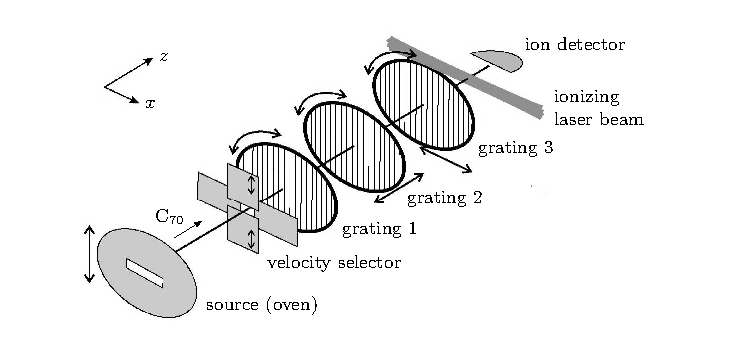
\includegraphics[width=.85\linewidth]{figures/ch06_fig09.pdf}
\caption{Zeilingerのグループの実験\cite{ref264,ref265,ref266,ref267}で、$\mathrm C_{70}$分子の物質波干渉を観測する配置。許可を得て\cite{ref264}の図を改作。Copyright 2002 by the American Physical Society.}
\end{figure}

装置を通る分子の平均速度は、分子源の位置を変え、自由飛行放物線を描くビームの異なる部分を、固定高さの制限器で選ぶことで、約90から$220\,\mathrm{m/s}$の間で調整できる。これらは、de Broglie波長2から6pmに対応する。分子と他粒子の衝突を最小にするため、装置全体は真空槽に収められている。

\subsubsectionlink{重い分子の波動性を確かめる}
典型的な実験一回の結果を図6.10に示す。横軸は走査マスクの$x$軸方向の位置（図6.9参照）、縦軸は各位置における格子後方の分子密度である。$\mathrm C_{70}$分子密度の振動が明瞭に見え、空間的コヒーレンスと干渉効果の存在を確認できる。
% 原文 p.263
\hypertarget{srcpage:263}{}\label{srcpage:263}
分子速度を変え、Talbot--Lau理論に一致する密度模様の変化を観測することで、この模様が実際にTalbot--Lau効果によることも明示的に確認された。
\begin{figure}[htbp]\centering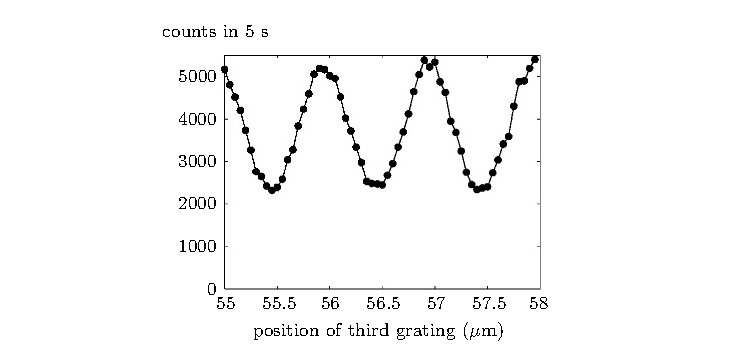
\includegraphics[width=.82\linewidth]{figures/ch06_fig10.pdf}
\caption{Zeilingerのグループの実験で観測された、$\mathrm C_{70}$分子の干渉縞。実線は理論予測に基づいて当てはめた正弦曲線である。許可を得て\cite{ref264}の図を改作。Copyright 2002 by the American Physical Society.}
\end{figure}

また、干渉効果は厳密な一粒子効果であり、異なる分子間の干渉によるものではない。理由は二つある。第一に、粒子間干渉には、相互作用する分子が同じ状態である必要がある。しかし、各$\mathrm C_{70}$分子は非常に多数の内部自由度を持つため、その可能性は実効的にゼロである。第二に、二分子間の距離は、いかなる分子間力の範囲よりもはるかに大きく、したがって、本質的に、どの瞬間にも装置を通っているのは単一分子だけである。

\subsubsectionlink{経路情報とデコヒーレンス}
それでは、本章の主要主題である、デコヒーレンスの実験観測へ移ろう。$\mathrm C_{70}$干渉実験では、デコヒーレンスは主として、分子と背景気体の分子の衝突による。真空は完全ではないので、背景気体は装置内にある程度常に存在する。このような衝突デコヒーレンスは第3章で詳しく述べ、自然界に普遍的にある源であることを示した。しかし、本章冒頭で述べたように、中間的尺度や巨視的物体では、それが通常あまりに速く、その漸進的作用を観測することは実効的に不可能である。
% 原文 p.264
\hypertarget{srcpage:264}{}\label{srcpage:264}
ここに、$\mathrm C_{70}$干渉実験の主要な利点がある。背景気体密度を変えることで、衝突デコヒーレンスの量を精密に調整できる。図6.11は、Lucia Hackermüllerら\cite{ref268}が報告した、背景気体の二つの圧力、すなわち密度で実験的に測定された干渉模様である（\cite{ref265}も参照）。左の図では、干渉縞が明瞭に見える。背景気体の圧力を高めると、縞が目立たなくなる（右）。圧力$p$における干渉模様の可視度$V(p)$を、その最大振幅$c_{\max}(p)$と最小振幅$c_{\min}(p)$の相対差として定量化しよう。
\begin{equation}V(p)=\frac{c_{\max}(p)-c_{\min}(p)}{c_{\max}(p)+c_{\min}(p)}.\tag{6.30}\end{equation}
デコヒーレンスも他の実験的不完全さもない理想的場合には、$c_{\min}=0$で、完全な可視度を得る。完全にデコヒーレンスした場合、干渉模様は観測できず、$c_{\max}=c_{\min}$となるので、可視度はゼロである。

気体圧力$p$に対する可視度(6.30)の変化の実験データ\cite{ref265,ref268}を、図6.12に示す。可視度は$p$とともに指数関数的に低下する。縦軸が対数目盛であることに注意されたい。この指数減衰は、理論計算\cite{ref160,ref269}と見事に一致する。
\begin{figure}[htbp]\centering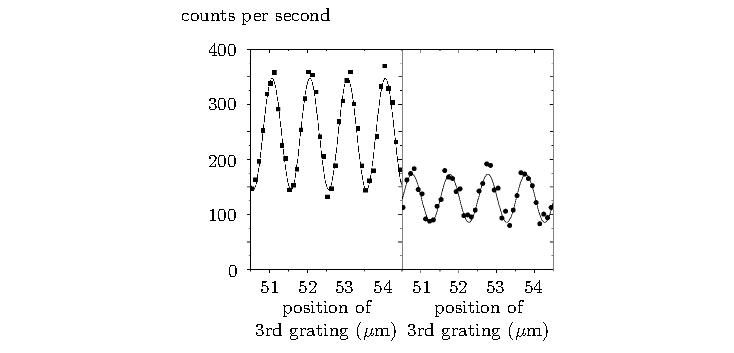
\includegraphics[width=.86\linewidth]{figures/ch06_fig11.pdf}
\caption{Zeilingerのグループの実験\cite{ref268}で観測された、背景気体分子との衝突が誘起するデコヒーレンスによる、$\mathrm C_{70}$分子干渉の減少。左から右へ気体圧力を高めると、干渉縞の可視度が低下する。Springer Science and Business Mediaのご厚意により、許可を得て\cite{ref268}の図を改作。}
\end{figure}
% 原文 p.265
\hypertarget{srcpage:265}{}\label{srcpage:265}
\begin{figure}[htbp]\centering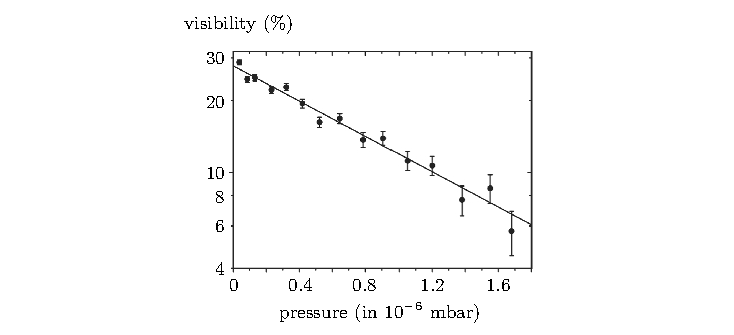
\includegraphics[width=.82\linewidth]{figures/ch06_fig12.pdf}
\caption{Zeilingerのグループ\cite{ref268}が報告した、背景気体圧力への干渉模様の可視度(6.30)の依存性。測定値（円）は、圧力に対する指数減衰を記述する理論予測（実線）によく一致する。Springer Science and Business Mediaのご厚意により、許可を得て\cite{ref268}の図を改作。}
\end{figure}
したがって、これらの実験は、干渉の観測に必要な量子コヒーレンスを、環境との相互作用が徐々に非局在化する様子を、印象的かつ直接に示す。この過程は完全に制御されている。たとえば背景気体の密度を変え、環境が得る経路情報量を変化させれば、デコヒーレンスの量、したがって量子的特徴の喪失を、精密に調整できる。こうして、量子・古典境界を滑らかに行き来して探索でき、観測が理論予測と極めてよく一致することが分かる。

\subsubsectionlink{熱放射の放出によるデコヒーレンス}
巨視的物体の最も重要なデコヒーレンス機構は何だろうか。これまで見たように、光子や空気分子など、他粒子との衝突は確かに普遍的にあり、決定的な役割を果たす。しかし、この長さ尺度でのもう一つの基本的な源は、熱放射の放出である。どの「大きな」物体も、多数の内部自由度へエネルギーを蓄えられる。巨視的物体は、本質的に絶えず光子を吸収し放出する。各放出光子は、物体の経路の情報を運び去り、位置基底でのデコヒーレンス、したがって物体の空間的局在化を生じさせる。

巨視的物体では、熱放射の放出は通常、空間的干渉効果を観測する可能性を完全に閉ざすほど強い。興味深いことに、以下で見るように、$\mathrm C_{70}$分子は、熱的デコヒーレンスに関して微視的領域と巨視的領域の境界を、ちょうどまたいでいる。
% 原文 p.266
\hypertarget{srcpage:266}{}\label{srcpage:266}
可視の干渉模様を生じさせるほど小さい一方、十分複雑であるため、数千Kまで加熱すると、熱的デコヒーレンスによって干渉模様が完全に消える。したがって、これらの分子は、熱的デコヒーレンス効果を明示的に観測するのに理想的である。装置を通過する前に徐々に加熱し、分子温度の関数として干渉縞の可視度の減衰を記録すればよい。

この考えは、Zeilingerのグループが行い、Hackermüllerら\cite{ref267}が2004年に報告した、注目すべき実験で実現された。格子を通る前に、$\mathrm C_{70}$分子は、レーザービームによって、源での約900Kから約3000Kまで加熱された。四つのレーザー出力、したがって分子平均温度について観測された干渉模様を、図6.13に示す。

予想どおり、分子からの熱放射のため、レーザー出力とともに可視度が低下する。さまざまな加熱出力での一連の実験結果を図6.14に示す。実験データは、理論計算\cite{ref267}の予測によく一致する。
\begin{figure}[htbp]\centering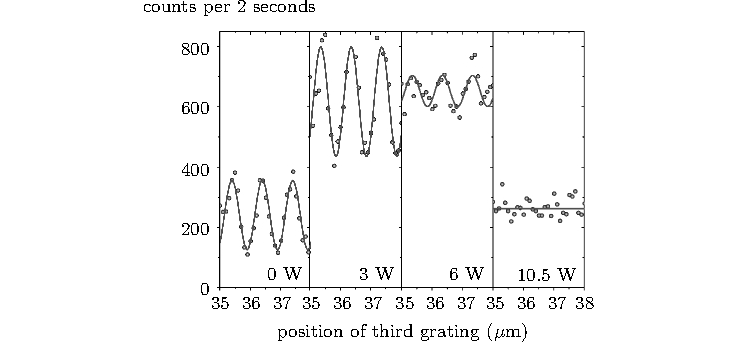
\includegraphics[width=.96\linewidth]{figures/ch06_fig13.pdf}
\caption{Hackermüllerら\cite{ref267}の実験で測定された、異なるレーザー加熱出力、したがって異なる分子平均温度における、$\mathrm C_{70}$分子の干渉模様。平均温度が上がるほど可視度が低下する。異なる加熱出力で全体の平均計数率が変わるのは、分子エネルギーによるイオン計数検出器の効率の変化と、加熱段階での電離・破砕効果による。Macmillan Publishers Ltdの許可を得て\cite{ref267}から転載：Nature, copyright 2004.}
\end{figure}
% 原文 p.267
\hypertarget{srcpage:267}{}\label{srcpage:267}
\begin{figure}[htbp]\centering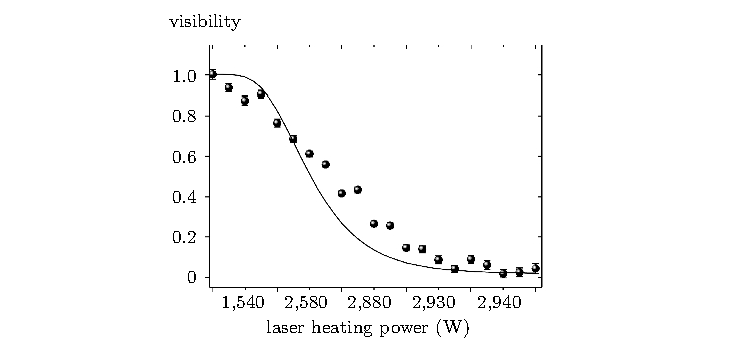
\includegraphics[width=.85\linewidth]{figures/ch06_fig14.pdf}
\caption{Hackermüllerら\cite{ref267}の実験における、レーザー加熱出力と平均分子温度の関数としての、$\mathrm C_{70}$干渉模様の可視度の減衰。円は実験データを表し、実線の理論予測によく一致する。Macmillan Publishers Ltdの許可を得て\cite{ref267}から転載：Nature, copyright 2004.}
\end{figure}
さらに詳しい実験の理論解析は、\cite{ref270,ref271}にある。

結果は、$\mathrm C_{70}$分子が約1000K以下なら、熱的デコヒーレンスは、干渉模様を観測できるほど弱いことを示す。約2000K以上では可視度を有意に低下させ、約3000Kで干渉模様は完全に消える。

これは次のように説明できる。放出光子が、$\mathrm C_{70}$分子の経路を分解できるだけの経路情報を伝えるには、その波長は、分子の異なる経路の隔たり、すなわち回折格子の異なるスリットの通過に対応する波束の極大間隔と、同程度でなければならない。この隔たりはスリット自体の間隔$d\approx1\,\mu\mathrm m$程度なので、熱的デコヒーレンスには、波長$\lambda\lesssim1\,\mu\mathrm m$の光子放出が必要である。分子がこの波長の光子を放出する有意な確率が現れるのは、2000Kを超える温度になってからだと分かる。約3000Kでは、典型的に、そのような光子を数個放出する。これが、干渉模様を完全に破壊するのに十分な経路情報を、環境へ移す。

\subsubsectionlink{バッキーボールを超えて}
$\mathrm C_{70}$分子の一粒子干渉縞が実験で観測された以上、自然な次の段階は、ますます大きな分子で、そのような量子効果を示すことである。
% 原文 p.268
\hypertarget{srcpage:268}{}\label{srcpage:268}
実際、Zeilingerのグループは、Hackermüllerらが2002年に報告した実験\cite{ref266}で、すでに次の一歩を踏み出した。$\mathrm C_{70}$用と同様の配置で、さらに重いフッ素化フラーレン$\mathrm C_{60}\mathrm F_{48}$（質量$m=1632\,\mathrm{amu}$、108原子）と、生体分子テトラフェニルポルフィリン$\mathrm C_{44}\mathrm H_{30}\mathrm N_4$（質量$m=614\,\mathrm{amu}$、幅2nm以上）の干渉模様が観測された。分子構造を図6.15、得られた干渉模様を図6.16に示す。これらの比較的重く複雑な分子でも、明確な干渉縞が観測され、可視度は理論予測によく一致した。
\begin{figure}[htbp]\centering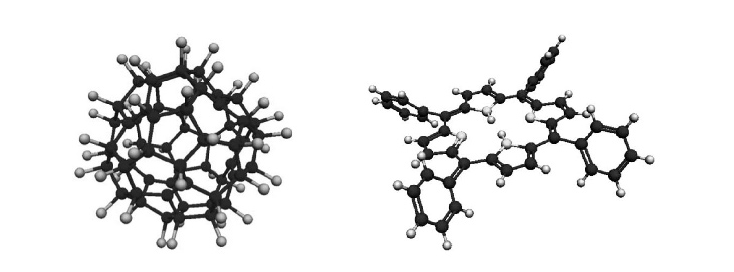
\includegraphics[width=.9\linewidth]{figures/ch06_fig15.pdf}
\caption{Hackermüllerら\cite{ref266}の干渉実験に用いられた、$\mathrm C_{60}\mathrm F_{48}$分子（左）と、生体分子テトラフェニルポルフィリン$\mathrm C_{44}\mathrm H_{30}\mathrm N_4$（右）の三次元構造。許可を得て\cite{ref266}から転載。Copyright 2003 by the American Physical Society.}
\end{figure}
\begin{figure}[htbp]\centering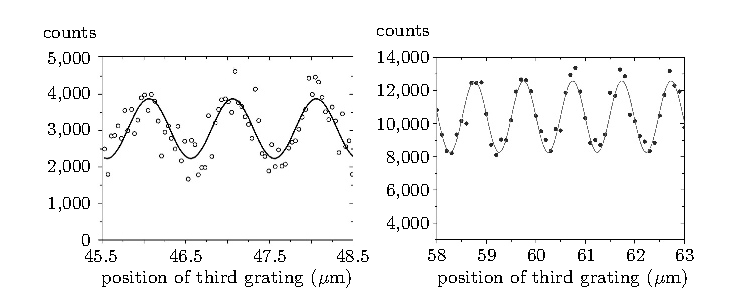
\includegraphics[width=.96\linewidth]{figures/ch06_fig16.pdf}
\caption{Hackermüllerら\cite{ref266}の実験で観測された、$\mathrm C_{60}\mathrm F_{48}$分子（左）と、生体分子テトラフェニルポルフィリン$\mathrm C_{44}\mathrm H_{30}\mathrm N_4$（右）の干渉縞。実線は当てはめた正弦曲線。許可を得て\cite{ref266}の図を改作。Copyright 2003 by the American Physical Society.}
\end{figure}

% 原文 p.269
\hypertarget{srcpage:269}{}\label{srcpage:269}
さらに大きい粒子、たとえばタンパク質やウイルスなどの生体分子\cite{ref268,ref272}、炭素質エアロゾル\cite{ref271}を使う干渉実験の実現可能性も、推測できる。そのような実験は、主に三つの要因で制限される。
\begin{enumerate}
\item 衝突デコヒーレンス。これらの分子の干渉縞を観測するには、装置内の真空が非常によくなければならない。背景気体密度の関数として干渉縞の可視度を記述するデコヒーレンス模型を使い、ライノウイルスの大きさに至るまでの、いくつかの生体分子について、干渉の観測に必要な真空の質が評価された\cite{ref268,ref272}（図6.17参照）。この評価は、現在の約3倍である、格子間隔1mの長いTalbot--Lau干渉計を使えることを仮定するが、これはまだ実験的に実現されていない。この設計なら、必要な低い背景気体密度は、現在の技術で達成できる範囲にある\cite{ref265,ref268}。
\item 熱的デコヒーレンス。大きな尺度では、これがますます重要になる。たとえば、Talbot--Lau干渉計とは異なる単純な二重スリット配置では、小さなウイルス（質量$5\times10^7\,\mathrm{amu}$）が、十分な可視度の干渉模様を示すには、約40Kまで冷却する必要があると評価された\cite{ref271}。そのような「冷たいウイルス」のビームを実験室で作るのは、明らかにかなり難しい。ゆえに、$\mathrm C_{70}$より大きい物体では、
% 原文 p.270
\hypertarget{srcpage:270}{}\label{srcpage:270}
衝突デコヒーレンスよりも、熱的デコヒーレンスの影響を弱める方が、実験的にははるかに難しくなるかもしれない\cite{ref271}。
\item 慣性力と振動による位相緩和。それ自体はデコヒーレンス効果ではないが、地球の質量と回転、回折格子の振動によって誘起される、重力的、回転的、音響的擾乱の雑音も、可視度へ影響する\cite{ref273}。これらは干渉縞の観測可能性を強く制限し得るので、実験者は、ここで述べたTalbot--Lau配置で、これらの雑音源を最小にすることに大きな注意を払っている。それでも、図6.17の粒子では、振動雑音が干渉観測の大きな障害になると予想される\cite{ref273}。現在利用できる配置では、その雑音は、衝突・熱的デコヒーレンス以上に、可視度を低下させる可能性が高い。
\end{enumerate}
\begin{figure}[htbp]\centering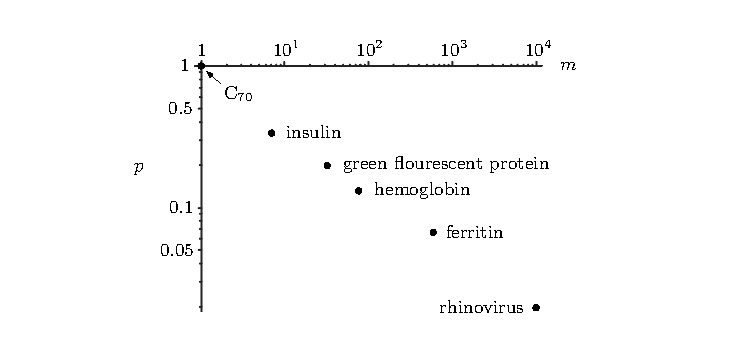
\includegraphics[width=.85\linewidth]{figures/ch06_fig17.pdf}
\caption{長いTalbot--Lau干渉計で、いくつかの生体分子の干渉縞を観測できる、背景気体の最大圧力$p$の評価。横軸は$\mathrm C_{70}$分子の質量を基準とする分子量$m$。縦軸の圧力は、$\mathrm C_{70}$の干渉観測に必要な圧力で規格化している。Hackermüllerら\cite{ref268}のデータから作図。}
\end{figure}

しかし、念頭に置くべき重要な点は、理論的デコヒーレンス模型を用い、干渉効果を観測する条件を精密に指定し定量化できることである。Copenhagen解釈が仮定するような、曖昧に定義された、量子領域と古典領域の基本的区分という仮定に、もはやとどまる必要はない。代わりに、対象分子を環境と相互作用する開いた量子系として扱うことで、干渉を観測するために何をすべきか、特定の実験設定でなぜ干渉縞が観測できないかを、理解できる。

$\mathrm C_{70}$分子は、周囲の粒子との衝突と熱放射の放出によるデコヒーレンスの、漸進的作用の観測を可能にする、ちょうどよい感受性を持つ。したがって、系を古典領域へ導くデコヒーレンスの、直接的で制御可能な影響を示す、これ以上分かりやすく直観的な実験を想像することは難しい。将来の干渉実験は、その限界をさらに巨視的領域へ押し進めると期待され、この分野の研究の進展を追うのは楽しみである。

\subsectionlink{SQUIDとその他の超伝導量子ビット}
それでは、超伝導量子二状態系、すなわち量子ビット系へ移ろう。過去10年、これらは巨視的なコヒーレンスとデコヒーレンスの実験研究で、中心的な役割を担うようになった。超伝導量子コンピューターの構成要素となる可能性も、その重要性を高めている\cite{ref274}。以下では、いわゆる超伝導量子干渉素子、略してSQUIDに焦点を当てる。Cooper対箱など、関連する他の型の超伝導量子ビット系にも触れる。

SQUIDは、さまざまな魅力的な量子効果を示せる巨視的量子系である。SQUIDでは、Bose凝縮した何十億もの電子対（以下参照）の状態が、
% 原文 p.271
\hypertarget{srcpage:271}{}\label{srcpage:271}
Schrödinger方程式に従って発展する、単一の集団的な巨視的変数で記述される。量子領域と、量子力学の限界の可能性を探索するSQUIDの潜在力は、早くから認識された。1980年、Leggett\cite{ref275}は、巨視的系で量子コヒーレントな振る舞いが可能であることを示すため、SQUIDの巨視的磁束状態の重ね合わせを含む思考実験を提案した。しかし、この提案が実験で成功するまでには、20年を要した\cite{ref276,ref277}。

\subsubsectionlink{超伝導と超電流}
超伝導現象は、1900年代初めにHeike Kamerlingh Onnesが初めて発見した。Onnesは液体Heで固体Hgを冷却し、絶対零度より数K高い温度で、Hgの電気抵抗が消えることを見いだした。1911年、「水銀の抵抗が消失する際の急激な速度について」という、適切な題名の論文\cite{ref278}で結果を公表した。2年後、この研究に対してNobel賞を授与された。しかし、微視的水準での理論的理解が得られたのは、1957年、Bardeen、Cooper、Schrieffer\cite{ref279}が、物質の結晶格子中のフォノンを介した相互引力により、逆向きのスピンを持つ電子が、いわゆるCooper対を形成することとして超伝導を説明してからであった。Cooper対は実効的にボソンとして働くため、フェルミオンである単一電子とは、著しく異なる性質を示せる。

Cooper対が、何の抵抗も受けずに物質を通過できるのは、なぜだろうか。各対は、第一励起状態からエネルギーギャップ$\Delta E$で隔てられた低エネルギー基底状態に対応することに注意しよう。結晶格子の熱振動エネルギーが$\Delta E$未満なら、格子は対の状態に遷移を誘起できず、対は格子との衝突で影響を受けない。これは、任意量のエネルギーを吸収・放出して散逸、したがって電気抵抗を生じさせる、単一の自由電子と対照的である。

超伝導の主要な特徴は、Cooper対がすべて同じ低エネルギー量子状態を取るため、多数の対が、対の集団的な重心運動を単一の巨視的波動関数で表す、無抵抗電流、すなわち「超電流」を形成できることである。量子力学の特異な特徴によって、そのような電流の流れには、外部電圧さえ必要ない。二つの超伝導物質の間に、非常に薄い絶縁障壁を入れるだけでよい。Cooper対はその障壁をトンネル通過し、電圧ゼロで超電流が流れる。この、実験的によく検証された純粋に量子力学的な現象は、いわゆるJosephson効果の、いくつかの形の一つであり、
% 原文 p.272
\hypertarget{srcpage:272}{}\label{srcpage:272}
障壁は対応してJosephson接合と呼ばれる（総説は\cite{ref280,ref281}参照）。

\subsubsectionlink{SQUIDの基本的物理}
SQUIDは、Josephson効果に直接基づく。超伝導物質の環に、一つ（rf-SQUID）または複数（dc-SQUID）のJosephson接合を入れたものである（図6.18）。本節では、単一接合のrf-SQUIDに焦点を当てる。接合を通るCooper対の量子トンネルによって、環に沿って超電流が流れ、SQUID環を貫く磁束が生じる。また、強度を調節できる外部磁場中にSQUIDを置き、追加の磁束$\Phi_{\mathrm{ext}}$を環へ与える。この外部磁束の目的は、後に説明する。

量子力学は、超電流を記述する波動関数が環に沿って連続であること、したがって波長の整数倍が環の周長に等しいことを要求する。環を一周する全位相変化は、$2\pi\Phi/\Phi_0$である。ここで$\Phi_0=h/(2e)$は、いわゆる磁束量子で、$e$は電子電荷である。$\Phi$は、超電流が作る磁束と外部磁場による$\Phi_{\mathrm{ext}}$からなる、環を貫く全捕捉磁束を表す。環にJosephson接合がなければ、波動関数の連続性は、条件
\begin{equation}\Phi/\Phi_0=k,\qquad k=1,2,\ldots\tag{6.31}\end{equation}
となる。しかしJosephson接合は、その物理的性質で完全に決まる、追加の位相シフト$\Delta\phi_{\mathrm J}$を導入する。位相連続性の完全な条件は、
\begin{equation}\Delta\phi_{\mathrm J}+2\pi\Phi/\Phi_0=2\pi k,\qquad k=1,2,\ldots .\tag{6.32}\end{equation}
\begin{figure}[htbp]\centering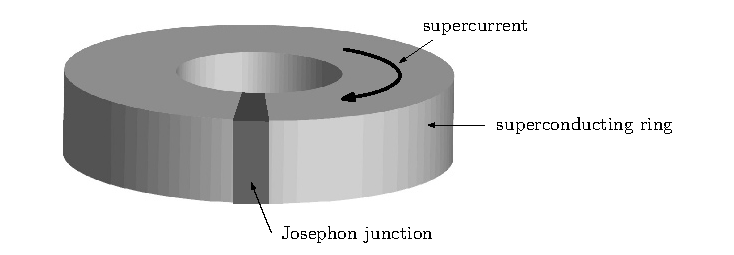
\includegraphics[width=.82\linewidth]{figures/ch06_fig18.pdf}
\caption{SQUIDの模式図。超伝導物質の環に一つまたは複数のJosephson接合を入れると、環に沿った無散逸の「超電流」が生じる。この超電流が、環を貫く磁束を作る。}
\end{figure}

% 原文 p.273
\hypertarget{srcpage:273}{}\label{srcpage:273}
$\Delta\phi_{\mathrm J}$と$\Phi_0$は固定されているので、(6.32)の唯一の自由パラメーターは全磁束$\Phi$である。したがってSQUIDでは、$10^9$個程度のCooper対という巨視的量の物質の動力学が、単一の巨視的座標$\Phi$の量子力学的発展によって、集団的に決定される。磁束が主要変数であるため、これらの素子はしばしば超伝導磁束量子ビットと呼ばれる。6.3.4節で述べるように、電荷や位相が主要変数となる、ほかの超伝導量子ビット系もある\cite{ref281}。

それでは、$\Phi$の動力学を論じよう。その発展は、次の形の有効Hamiltonianに従う。
\begin{equation}
H=\frac{P_\Phi^2}{2C}+U(\Phi)
=\frac{\hbar^2}{2C}\frac{\mathrm d^2}{\mathrm d\Phi^2}
+\left[\frac{(\Phi-\Phi_{\mathrm{ext}})^2}{2L}-\frac{I_c\Phi_0}{2\pi}\cos\left(2\pi\frac\Phi{\Phi_0}\right)\right].\tag{6.33}
\end{equation}
ここで$C$は全静電容量、$L$は環の自己インダクタンス、$I_c$はJosephson接合の臨界電流である。ここではこのHamiltonianの構造を導かない。関心のある読者は\cite{ref218}の導出を参照されたい。代わりに、それがどのような動力学を意味するのか、感覚をつかもう。

これは、ポテンシャル$U(\Phi)$中の、「質量」$C$を持つ仮想的「粒子」の運動を定めるHamiltonianと解釈できる。通常の正準変数である位置と運動量の役割は、ここでは全捕捉磁束$\Phi$と、その共役量$P_\Phi=-i\hbar\,\mathrm d/\mathrm d\Phi$が果たす。後者はしばしば全変位電流と呼ばれ、電荷の単位を持つ。実空間を動く粒子の運動エネルギーに相当するものは、ここでは静電エネルギーである。

外部磁場を調整し、誘起磁束$\Phi_{\mathrm{ext}}$をバイアス点$\Phi_{\mathrm{ext}}=\Phi_0/2$の近傍にすると、$U(\Phi)$は、傾いた一次元二重井戸ポテンシャルの形を取る（図6.19）。これが実験で関係する状況であり、以下ではこれを仮定する。傾きは$\Phi_{\mathrm{ext}}$によって決まり、$\Phi_{\mathrm{ext}}=\Phi_0/2$で、二重井戸は厳密に対称になる。この場合は後に詳しく論じる。したがって、外部印加磁場の強度で、ポテンシャルの形を変えられる。

大まかには、二つの井戸は、環を回る超電流の二方向、時計回りと反時計回りに対応する。各井戸は、接合による減衰が弱ければ、井戸間の障壁より十分低いところに局在する、Hamiltonian(6.33)のエネルギー固有状態$|k\rangle$をいくつか含む。こうして、環を回る古典的な持続時計回り電流、または反時計回り電流に、近似的に対応する、左井戸または右井戸のエネルギー固有状態の組を得る。

より正確には、波動関数$\psi_k(\Phi)\equiv\langle\Phi|k\rangle$は、局所的にs波型である。つまり、振幅は井戸の一方の底の周囲に狭いピークを持ち、
% 原文 p.274
\hypertarget{srcpage:274}{}\label{srcpage:274}
磁束空間での広がりが非常に小さい。したがって各$|k\rangle$は、全磁束$\Phi$の比較的狭い範囲に対応し、少なくとも十分小さな$k$では、磁束演算子の「ぼやけた」固有状態とみなせる。可能な離散磁束値は、連続性条件(6.32)で決まる。それゆえ$|k\rangle$は、しばしば「$k$フラクソイド状態」と呼ばれる。
\begin{figure}[htbp]\centering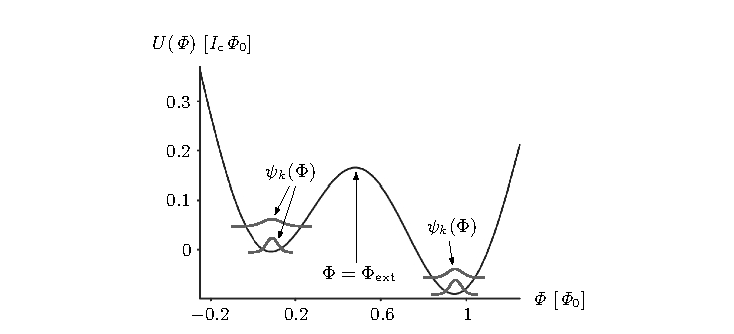
\includegraphics[width=.85\linewidth]{figures/ch06_fig19.pdf}
\caption{バイアス点$\Phi_{\mathrm{ext}}=\Phi_0/2$近傍の、SQUIDの有効二重井戸ポテンシャル$U(\Phi)$（単位$I_c\Phi_0$）。低いエネルギー固有状態$\psi_k(\Phi)\equiv\langle\Phi|k\rangle$は、各井戸の底近くによく局在し、したがって磁束演算子の近似的固有状態でもある。$\Phi$軸の単位は磁束量子$\Phi_0$で、$\Phi_{\mathrm{ext}}=3\Phi_0/5$とした。}
\end{figure}

古典的には、低い$k$フラクソイド状態$|k\rangle$のエネルギーは障壁高さ未満なので、二井戸を隔てる障壁を通過できない。しかし量子的には、井戸間の共鳴トンネルが起こり得る\cite{ref282,ref283}。たとえば放射場を加え、同じ井戸に局在する低い状態から高エネルギー状態へ系を励起すると、その状態は、その後、量子トンネルによって他方の井戸の、より低い、または等しいエネルギー準位へ減衰できる。これによって環を貫く磁束$\Phi$に巨視的変化が生じ、それが系の磁気モーメントの巨視的変化として観測できる。

通常SQUIDは、反対の井戸の底に局在する基底状態$|0\rangle$と第一励起状態$|1\rangle$が、より高い状態からエネルギー的によく分離するよう設計する。このとき、巨視的二状態系、すなわち量子ビットとして実効的に記述できる。基底には、超電流がそれぞれ確定した時計回りと反時計回りに流れる、二つの古典的持続電流状態$|\circlearrowright\rangle$、$|\circlearrowleft\rangle$を選ぶ。この二状態SQUIDの有効Hamiltonianは形式的に、
\begin{equation}\hat H=-\epsilon\hat\sigma_z-\Delta\hat\sigma_x.\tag{6.34}\end{equation}
% 原文 p.275
\hypertarget{srcpage:275}{}\label{srcpage:275}
と書ける。Pauliスピン演算子$\hat\sigma_z$の固有状態は$|\circlearrowright\rangle$、$|\circlearrowleft\rangle$であり、$2\epsilon=2I_p(\Phi_{\mathrm{ext}}-\Phi_0/2)$は、それらの非対称エネルギーを表す。$I_p\approx I_c$である。$\Delta$は二状態間のトンネル行列要素である。最低の二つのエネルギー固有状態$|0\rangle$、$|1\rangle$は、次の線形結合となる。
\begin{equation}|0\rangle=\cos\theta|\circlearrowright\rangle+\sin\theta|\circlearrowleft\rangle,\tag{6.35a}\end{equation}
\begin{equation}|1\rangle=-\sin\theta|\circlearrowright\rangle+\cos\theta|\circlearrowleft\rangle.\tag{6.35b}\end{equation}
ここで$\tan2\theta=\Delta/\epsilon$、エネルギーは$E_{0,1}=\mp\sqrt{\Delta^2+\epsilon^2}$である。したがって、$|0\rangle$と$|1\rangle$のエネルギー分裂は、$\Delta E=2E_1=2\sqrt{\Delta^2+\epsilon^2}$となる。バイアス点$\Phi_{\mathrm{ext}}=\Phi_0/2$から離れると、$\epsilon\gg\Delta$であり、$|\circlearrowright\rangle$、$|\circlearrowleft\rangle$は、それぞれゼロフラクソイド、1フラクソイドのエネルギー固有状態$|0\rangle$、$|1\rangle$と本質的に同一となる。これは上の議論に一致する。二状態$|0\rangle$、$|1\rangle$に対応する超電流の期待値は、$\pm I_p\cos2\theta$となることを示せる。正符号は時計回りを表す。

\subsubsectionlink{SQUIDの重ね合わせ状態とコヒーレント振動}
SQUIDがバイアス点$\Phi_{\mathrm{ext}}=\Phi_0/2$にあると何が起こるかを考えよう。二重井戸は対称になり、(6.34)で$\epsilon=0$となる。すなわち、左右の井戸のエネルギー準位がそろう。この場合、古典的には$|0\rangle$と$|1\rangle$の準位が交差し、縮退する。しかし量子的には、井戸間のトンネル障壁$\Delta$［(6.34)参照］が存続することで縮退が解ける。これが準位の「反発」をもたらし、反交差を生む（図6.20）。(6.35a)、(6.35b)では$\theta=\pi/4$なので、基底状態と第一励起状態は、持続電流状態の対称・反対称重ね合わせとなる。
\begin{equation}|0\rangle=\frac1{\sqrt2}(|\circlearrowright\rangle+|\circlearrowleft\rangle),\tag{6.36a}\end{equation}
\begin{equation}|1\rangle=\frac1{\sqrt2}(-|\circlearrowright\rangle+|\circlearrowleft\rangle).\tag{6.36b}\end{equation}
二つの新しい固有状態のエネルギー分裂$\Delta E$は、通常非常に小さく、接合の静電容量$C$だけで決まり、$\Delta E\propto e^{-\sqrt C}$とスケールする。

$|\circlearrowright\rangle$と$|\circlearrowleft\rangle$はそれぞれ左右の井戸に局在するので、重ね合わせ(6.36a)、(6.36b)は、二井戸にわたって非局在化している。この存在は、2000年、Friedmanら\cite{ref276}と、独立にvan der Walら\cite{ref277}が実験で確認した。Friedmanらの実験では、二状態はそれぞれ、何十億ものCooper対からなる、数$\mu\mathrm A$の逆方向の超電流に対応した。
% 原文 p.276
\hypertarget{srcpage:276}{}\label{srcpage:276}
これは、二電流の作る磁束に$\Phi_0/4$以上の巨視的差があることに当たり、局所磁気モーメントでは約$10^{10}\mu_{\mathrm B}$に等しい。$\mu_{\mathrm B}$はBohr磁子である。ゆえに、(6.36a)、(6.36b)は、20年前のLeggettの思考実験\cite{ref275}が描いたとおりの、巨視的に異なる状態のSchrödingerの猫型重ね合わせを表す。Friedmanらは、二状態間のエネルギー差$\Delta E$の静的分光測定という間接的方法で、存在を検証した。得られた$\Delta E$は、理論予測と極めてよく一致した。
\begin{figure}[htbp]\centering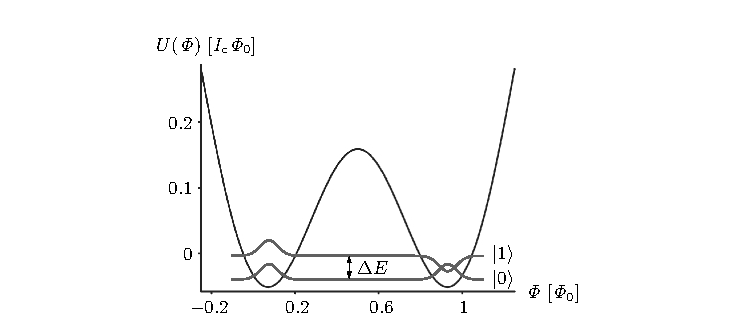
\includegraphics[width=.85\linewidth]{figures/ch06_fig20.pdf}
\caption{バイアス$\Phi_{\mathrm{ext}}=\Phi_0/2$でのSQUIDの有効ポテンシャル。この点で二重井戸は対称になる。トンネル障壁が井戸の準位交差を妨げ、非局在化した固有状態$|0\rangle=(|\circlearrowright\rangle+|\circlearrowleft\rangle)/\sqrt2$（新しい対称基底状態）、$|1\rangle=(-|\circlearrowright\rangle+|\circlearrowleft\rangle)/\sqrt2$（新しい反対称第一励起状態）の形成を介して、反交差が起こる。これらは「古典的」持続電流状態の重ね合わせである。存在は、分光測定\cite{ref276,ref277}とコヒーレントRabi振動の観測\cite{ref284,ref285}によって、実験的に確認された。}
\end{figure}

そのような重ね合わせの存在を示す別の方法は、持続電流状態間のコヒーレント振動を観測することである。これは6.1.1節のRabi型振動である。まず、SQUIDを貫く外部磁束を、縮退点$\Phi_{\mathrm{ext}}=\Phi_0/2$からわずかにずらし、エネルギー固有状態$|0\rangle$と$|1\rangle$を縮退近くにする。緩和させることで基底状態$|0\rangle$に初期化する。次に、二状態間の小さなエネルギー差$\Delta E$に周波数を合わせた、マイクロ波パルスを加える。Rabi振動の議論によれば、量子ビットは$|0\rangle$と$|1\rangle$の間、したがって持続電流状態間でも振動する［(6.35)参照］。
% 原文 p.277
\hypertarget{srcpage:277}{}\label{srcpage:277}
これは、巨視的超電流が環の時計回りと反時計回りの間で振動することとして現れる（図6.21）。振動はRabi周波数で起き、その周波数は量子ビットとマイクロ波場の結合強度で決まり、マイクロ波振幅に線形に依存する。したがって、SQUIDが二状態の各々にある相対確率は、パルスの振幅と長さに依存する［(6.8)参照］。

2003年、Chiorescuたち\cite{ref284}は、超伝導磁束量子ビットでこのRabi振動を実験的に示した。実験系は、三つのJosephson接合を入れた、$\mu\mathrm m$サイズの超伝導環からなる（図6.22）。単一接合のrf-SQUIDに比べ、三接合を使っても基本物理は大きく変わらないが、適切な調整が容易になる。量子ビットはさらに、Josephson接合を二つ持つdc-SQUIDに結合され、それが量子ビットの磁束を読む極めて高感度な装置として働く。

Chiorescuらは、与えられた長さと振幅のマイクロ波パルスを加え、次に、実験で利用できる観測量に対応する、持続電流基底$\{|\circlearrowright\rangle,|\circlearrowleft\rangle\}$で射影測定を行った。
\begin{figure}[htbp]\centering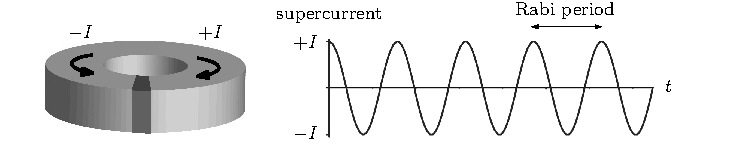
\includegraphics[width=.9\linewidth]{figures/ch06_fig21.pdf}
\caption{縮退点$\Phi_{\mathrm{ext}}=\Phi_0/2$の近くに調整したSQUIDの量子コヒーレントなトンネルは、巨視的超電流が時計回りと反時計回りの間でコヒーレントに振動することによって観測できる。}
\end{figure}
\begin{figure}[htbp]\centering
\includegraphics[width=.9\linewidth]{figures/ch06_fig22.pdf}
\caption{Chiorescuら\cite{ref284}の実験に使われた超伝導磁束量子ビット。右側の実際の量子ビットは、三つのJosephson接合を持つ小さな超伝導環である。白黒の矢印は持続電流の二方向を示す。量子ビットと一部を共有する、より大きい超伝導環に二接合を入れたSQUIDが、磁束の変化を検出する。許可を得て\cite{ref284}から転載。Copyright 2003 by AAAS.}
\end{figure}
% 原文 p.278
\hypertarget{srcpage:278}{}\label{srcpage:278}
この手順を数千回行い、たとえば超電流が時計回りとなる$|\circlearrowright\rangle$状態に、量子ビットを見いだす実験的確率を得た。マイクロ波振幅を固定し、パルス長を変えて繰り返すと、約150nsという驚くほど長い減衰時間を持つ、数百回の減衰Rabi振動を追跡できた（図6.23）。それが実際にRabi型の量子コヒーレント振動であると確認するため、研究者たちは、観測された周波数がマイクロ波振幅に線形比例することを検証した。これはRabi過程の主要な特徴である。別の連続読出し方式は、その後のIlichevら\cite{ref285}の実験で実現された。

Chiorescuら\cite{ref284}とIlichevら\cite{ref285}のRabi振動は、以前のFriedmanら\cite{ref276}とvan der Walら\cite{ref277}の分光結果とともに、巨視的に異なる超電流状態のコヒーレントな重ね合わせの存在を、印象的に示す。
\begin{figure}[htbp]\centering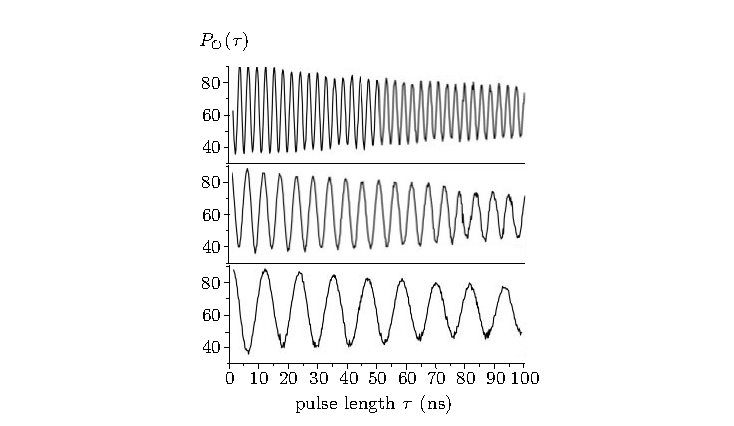
\includegraphics[width=.8\linewidth]{figures/ch06_fig23.pdf}
\caption{Chiorescuら\cite{ref284}の実験で観測された、超伝導磁束量子ビットの巨視的な逆方向超電流状態$|\circlearrowright\rangle$と$|\circlearrowleft\rangle$の間のRabi振動。これは二状態のコヒーレント重ね合わせを確認する。共鳴マイクロ波の三つの振幅の結果を示し、上から下へ振幅が小さくなる。縦軸は、特定の確定電流状態、たとえば$|\circlearrowright\rangle$に見いだされた実験の割合$P_{\circlearrowright}(\tau)$（\%）を、パルス長$\tau$の関数として示す。許可を得て\cite{ref284}の図を改作。Copyright 2003 by AAAS.}
\end{figure}
% 原文 p.279
\hypertarget{srcpage:279}{}\label{srcpage:279}
SQUIDは、この種の重ね合わせ状態の生成に特に適している。SQUID環を貫く捕捉磁束という、関係する巨視的変数を、Josephson接合の微視的なエネルギー差で制御できるからである\cite{ref286}。トンネル障壁の高さ$\Delta$は、環の大きさとは独立に、主として接合の性質で決まる。これは、達成可能な巨視的磁束状態の重ね合わせの「大きさ」が、異なりの程度そのもの、すなわち持続電流状態間の磁束差に、弱くしか依存しないことを意味する。

この特徴によって、ほかの実験で達成したものよりも、巨視的な異なりの程度がはるかに大きい「古典的」状態の重ね合わせを作れる。たとえば$\mathrm C_{70}$分子の物質波回折実験（6.2節）では、回折模様を観測するため、分子中の原子数$N$に伴って、回折格子の間隔を$1/\sqrt N$に従って減らす必要がある。したがって、この場合、ある大きさの分子の干渉模様を実験で作る能力は、分子の大きさ自体に応じて変わる。

\subsubsectionlink{デコヒーレンスを観測し定量化する}
振動する占有確率の包絡線の減衰（図6.23参照）から導かれる、Rabi振動の特徴的減衰時間は、持続電流重ね合わせ(6.36a)、(6.36b)に固有のデコヒーレンス時間尺度を、直ちに与えるわけではないことに注意が必要である。Rabi振動は、加えたマイクロ波パルスという外部駆動場によって誘起されるためである。しかしデコヒーレンス時間を測るには、制御されない環境と相互作用する量子ビットが、自由に、すなわち駆動なしで発展する間に、重ね合わせ成分間の相対位相情報が非局在化することを考えなければならない。

この目標は、Ramsey干渉法\cite{ref051}で達成できる。以下の手順は、2.2.2節で述べた「共鳴」Ramsey法の変形である。まず、量子ビットを縮退点$\Phi_{\mathrm{ext}}=\Phi_0/2$近くに設定し、再びエネルギー基底状態$|0\rangle$に初期化する。次に、二準位間の遷移周波数$\Delta E/(2\pi)$から$\delta f$だけ離調した、$\pi/2$マイクロ波パルスを加える。これにより$|0\rangle$と$|1\rangle$のコヒーレント重ね合わせへ変換し、時間$\tau$だけ自由に発展させる。この間、加えたマイクロ波周波数で回転する座標系では、相対位相が$2\pi(\delta f)\tau$だけ増す。その後、第二の非共鳴$\pi/2$パルスを加える。得られる重ね合わせでは、$|0\rangle$と$|1\rangle$の係数の大きさが、周波数$\delta f/2$で、遅延時間$\tau$に振動的に依存する。したがって、古典的な持続電流状態の占有確率は、
% 原文 p.280
\hypertarget{srcpage:280}{}\label{srcpage:280}
周波数$\delta f$で、$\tau$の関数として振動する。

実際には、量子ビットの自由発展時間$\tau$の間に、デコヒーレンスが二つのエネルギー状態、したがって持続電流状態間のコヒーレンスを減らすので、振動振幅は減衰すると予想する。2.2.2節で説明したように、完全にデコヒーレンスすると、占有確率が$\tau$に依存しない、持続電流状態の非コヒーレント混合へ至る。

遅延時間を増すと占有確率の振動がやがて消えることにより、デコヒーレンスの漸進的効果を観測し、定量化できる。Chiorescuら\cite{ref284}は、さまざまな遅延時間で、持続電流状態の関係する占有確率を測った。その減衰振動を追い、特徴的デコヒーレンス時間尺度を読み取った（図6.24）。

予想された、遅延時間への振動的依存性が見られる。振動周波数はマイクロ波の離調$\delta f$に一致し、Ramsey理論の予測と極めてよく一致した。包絡線の減衰から約20nsのデコヒーレンス時間を得た。これは、この実験で量子ビットが自由発展する間に、古典的な持続電流状態間の位相コヒーレンスが、環境によって失われる特徴的時間尺度である。

より最近の磁束量子ビット実験では、最大$4\,\mu\mathrm s$という、はるかに長いデコヒーレンス時間が観測された\cite{ref287}。この有望な結果は、超伝導量子ビットが固体量子計算素子の実現に適するかもしれないという期待を高めた（第7章参照）。制御パルスによるゲート操作は非常に速く、単一量子ビットゲート操作は約2nsで行える。
\begin{figure}[htbp]\centering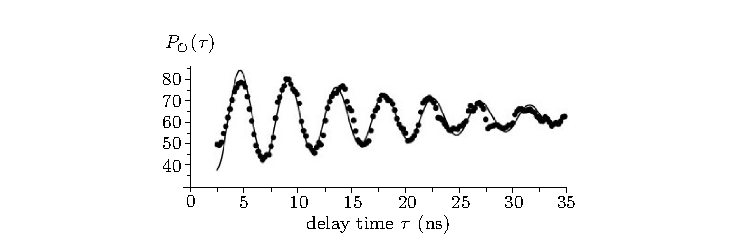
\includegraphics[width=.85\linewidth]{figures/ch06_fig24.pdf}
\caption{Chiorescuら\cite{ref284}の実験で観測された、超伝導磁束量子ビットへの二つの$\pi/2$パルスの遅延時間$\tau$に対する、占有確率$P_{\circlearrowright}(\tau)$の依存性。振動振幅の減衰は、系からの漸進的なコヒーレンスの喪失に対応する。許可を得て\cite{ref284}の図を改作。Copyright 2003 by AAAS.}
\end{figure}
% 原文 p.281
\hypertarget{srcpage:281}{}\label{srcpage:281}
したがって、コヒーレンスを相当失うまでに、1000回程度のゲート操作が可能かもしれない。しかし、単純な量子アルゴリズムにも必要な$O(100{,}000)$回には、まだかなり遠い。

SQUIDの磁束変数の代わりに、電荷または位相を主要変数とする超伝導素子でも、量子コヒーレント振動とデコヒーレンスが観測されている。一般に、超伝導電荷・位相素子の物理の形式的記述は、上述のSQUIDとよく似ている。

一般にCooper対箱として知られる超伝導電荷量子ビットは、貯蔵庫からJosephson接合を通ってCooper対がトンネルできる、小さな超伝導「島」からなる。二つの量子ビット基底は、少なくとも一つのCooper対だけ異なる、島の二つの電荷状態に対応する。Cooper対箱は、電荷状態間のRabi振動を実験観測できた、最初の超伝導量子ビット系であり、1999年にNakamura、Pashkin、Tsai\cite{ref288}が達成した。2002年にはVionら\cite{ref289}が、$0.5\,\mu\mathrm s$のデコヒーレンス時間を持つ、数千回のコヒーレント振動を報告した。

Rabi型のコヒーレント振動は、位相量子ビットでも観測された。位相量子ビットはrf-SQUIDと同様、単一のJosephson接合を含む。ただし、環を貫く磁束の代わりに、主要変数は接合電極間の位相差である。Yuら\cite{ref290}は、巨視的に異なる位相状態間のRabi振動を測り、最大数$\mu\mathrm s$のデコヒーレンス時間を得た。Martinisら\cite{ref291}も、同様の結果を報告した。

現在の実験的証拠（たとえば\cite{ref291,ref292}参照）は、超伝導量子ビットのデコヒーレンスの主な源が、予想されそうな、環・接合系を制御する外部回路との相互作用ではなく、Josephson接合と超伝導体の内部欠陥の存在であることを示す。これらの欠陥は、しばしば有効二準位系として模型化できる。5.1.2節で触れたように、超伝導系などの低温系のデコヒーレンスと散逸が、主にこのような内部二準位系によることは、しばらく前から知られている\cite{ref199,ref200}。量子ビット自体が二準位系なので、そのデコヒーレンスの理論的記述に適切な模型は、5.4節のスピン・スピン型である可能性が高い\cite{ref199}。

たとえばMartinisら\cite{ref292}は、絶縁体のバルクとJosephson接合の両方にある二準位状態による誘電損失が生む、超伝導位相量子ビットのデコヒーレンス研究へ、この模型を適用した。理論研究から得た知見は、著しく改善された実験構造へ、成功裏に反映された。ほかの理論研究は、電流バイアスJosephson接合を制御するバイアス電流の揺らぎなど、雑音過程の影響を調べている\cite{ref293}。しかし、
% 原文 p.282
\hypertarget{srcpage:282}{}\label{srcpage:282}
2.12節の一般的議論（7.3節も参照）に照らすと、そのような雑音による集団の位相緩和と、環境とのもつれが生む「真の」デコヒーレンスを、明瞭に区別することが重要である。局所測定統計という現象論的視点では、両者が同様の結果を生むとしても、同じではない。
\subsectionlink{その他の実験領域}
前の各節では、中間的尺度および巨視的尺度で異なる状態の重ね合わせを生成・検出し、その漸進的デコヒーレンスを観測できた実験を述べた。これらでは、実験室で観測された量子から古典への現象を、デコヒーレンスが定性的・定量的に説明した。

同じように、ただし別の視点から、ある実験で重ね合わせ状態を生成・観測できない原因を理解するうえでも、デコヒーレンスは役立つ。本節では、現在までに得られたものよりも、さらに大きい非古典的重ね合わせを、将来生成・観測するための有望な候補となる、二つの実験領域を述べる。見るように、それらで重ね合わせの生成・観測がこれほど難しい理由を、デコヒーレンスによって定性的・定量的に記述できる。また、実験手順の改善方法を示唆し、実験室で望ましい重ね合わせを作る目標に、さらに近づくことも可能にする。

\subsubsectionlink{Bose--Einstein凝縮体におけるデコヒーレンス}
Bose--Einstein凝縮は、巨視的数の原子が、ある実験では最大$O(10^7)$個まで、量子相転移を起こし、すべての原子が個別性を失って同一量子状態を占める凝縮体となる、量子力学的現象である。したがって凝縮体は、位相を持つ単一の量子力学的$N$粒子波動関数で完全に記述できる。この位相は実験で調べられる。たとえば二つの凝縮体を重ねると、両者の位相差による干渉模様が観測される\cite{ref294,ref296,ref297,ref298,ref299}（図6.25）。最近は、単一凝縮体をコヒーレントに分割し、その後再結合して干渉縞を観測する干渉計も作れるようになった\cite{ref295}（同じく図6.25参照）。

このような量子的性質の実証の成功にもかかわらず、粒子数が巨視的に区別される状態の重ね合わせに、凝縮体を準備する実験は、いくつかの有望な理論提案\cite{ref300,ref301,ref302,ref303,ref304,ref305,ref306}があるにもかかわらず、これまで失敗している。
% 原文 p.283
\hypertarget{srcpage:283}{}\label{srcpage:283}
しかし、関係するデコヒーレンス機構を考慮すれば、この失敗は定性的にも定量的にもよく理解できる。凝縮体の重ね合わせ状態では、デコヒーレンスは主に、凝縮原子と非凝縮原子の間の、弾性・非弾性散乱によることが分かる。
\begin{figure}[htbp]\centering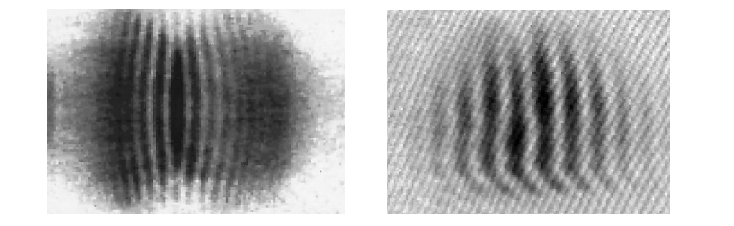
\includegraphics[width=.94\linewidth]{figures/ch06_fig25.pdf}
\caption{Bose--Einstein凝縮体の原子気体密度の干渉模様。左：独立な二凝縮体を重ねたときの、位相差による模様。許可を得て\cite{ref294}から転載。Copyright 1997 by AAAS. 右：凝縮体の「二重スリット」干渉計で得られた干渉縞。単一凝縮体をコヒーレントに分割し、通常の二重スリットの役割を模擬した後、再結合した。許可を得て\cite{ref295}から転載。Copyright 2004 by the American Physical Society.}
\end{figure}

この散乱過程の詳細な模型が作られ（たとえば\cite{ref102}参照）、凝縮体の大きさなどの主要実験パラメーターの関数として、デコヒーレンス時間尺度の現実的予測が得られる。また、これらの模型の知見は、巧妙な実験設計によってデコヒーレンスを最小にする具体的提案を生んだ。改善案には、デコヒーレンスを誘起する非凝縮原子の熱的雲を、より速く蒸発させる、修正した凝縮体トラップ\cite{ref102}、粒子数差状態ではなく相対位相状態の巨視的重ね合わせを作り、環境の選ぶ指針基底を考慮してデコヒーレンスを最小にすること\cite{ref303}、熱的雲の実効的大きさを減らす能動的な環境設計（7.5.3節）\cite{ref102}、重ね合わせ状態のより速い生成\cite{ref306}などがある。各提案は、特定の実験配置に関係する、さまざまなデコヒーレンス機構の分析から導かれる。配置が与えられると、模型は量子・古典境界の位置と、望ましい猫状態を実現するため、その境界を押し進めるには何ができ、何をすべきかを教える。

% 原文 p.284
\hypertarget{srcpage:284}{}\label{srcpage:284}
\subsubsectionlink{量子電気機械系におけるデコヒーレンス}
量子電気機械系、略してQEMSは、さらに大きい非古典的重ね合わせを生成する可能性を持つ、多彩な実験の仲間に、比較的最近加わったものである\cite{ref307}（入門は\cite{ref308,ref309}も参照）。QEMSには、デコヒーレンスと散逸の「振動子・スピン模型」との関連で、5.4.2節ですでに触れた。何十億もの原子が、空間中のよく区別できる二位置の重ね合わせにある、真に機械的な「Schrödingerの子猫」を示すために、QEMSは非常に有望である。この分野の急速な実験進展から、今後数年で、量子から古典への移行の探索で中心的な役割を果たす可能性が高い。

QEMSは、近年のナノテクノロジーの革命の成果である。主要部分は、シリコンなどの結晶材料から作る、小型の両端固定梁または片持ち梁で、典型寸法はnmから$\mu\mathrm m$程度である（図6.26）。梁は小さな機械的共振器として働く。短時間適切な駆動力を加えると、振動運動を始める。

寸法が極めて小さいため、機械系であることを考えると、振動周波数は驚くほど高くできる。最近の実験では、マイクロ波領域の1GHzまで達成した\cite{ref311}。また、共振器の散逸は比較的弱くでき、振幅が有意に減少するまでに、数万回自由振動する。運動は電子トランスデューサーで検出し、対応する電気信号へ変換して読み出す。
\begin{figure}[htbp]\centering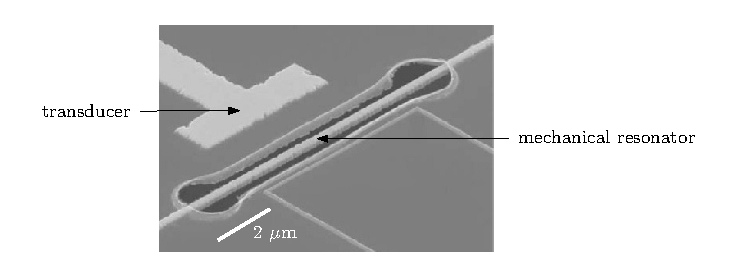
\includegraphics[width=.94\linewidth]{figures/ch06_fig26.pdf}
\caption{Cornell UniversityのKeith Schwabの研究室\cite{ref310}で作られた、量子電気機械系の実験的実現。幅200nm、長さ$8\,\mu\mathrm m$の梁が、固有周波数19.7MHzのナノ機械共振器として働く。電子トランスデューサーで、梁の振動を電気信号へ変換する。許可を得て\cite{ref310}から転載。Copyright 2004 by AAAS.}
\end{figure}
% 原文 p.285
\hypertarget{srcpage:285}{}\label{srcpage:285}
注目すべきことに、共振器の大部分の自由度は、QEMSの典型的動作温度であるmKという低温で「凍結」されるか、トランスデューサーへの結合が無視できる。したがって多くの場合、巨視的共振器は、梁の最低の基本曲げモードに対応する、単一の量子力学的調和振動子として実効的に扱える。QEMSのナノ機械共振器は、何十億もの原子からなり、多数の内部欠陥や不完全さで乱された、巨視的機械物体である。それにもかかわらず、これから述べるように、明確に量子力学的な効果を示せる。

QEMSの主要な特徴は、空間変位への極めて高い感度である。重要な量は、位置検出の量子限界を表す、調和振動子の量子零点変位の不確定性$\Delta x_{\mathrm{zp}}$である。現在実験室で作られるナノ機械共振器では、わずか0.1pm程度である\cite{ref307}。それでも最近の実験では、たとえば図6.26のQEMSを用い、$\Delta x_{\mathrm{zp}}$の数倍に至るまで空間変位を分解できた\cite{ref310}。したがって、量子限界での位置測定という目標に非常に近づいている。

\subsubsectionlink*{QEMSによる機械的「Schrödingerの子猫」の生成法}
研究者たちは、共振器を二つの異なる空間変位のコヒーレント重ね合わせに置き、その漸進的デコヒーレンスを観測する可能性も考えている。特に面白いのは、QEMSが、たとえば超伝導量子ビット（6.3節）やBose--Einstein凝縮体（6.4.1節）よりも、日常世界の物体にはるかに近い、純粋な機械構造であることだ。実現すれば、それは、巨視的で「粗い」通常物質の機械物体が、二つの異なる位置にある重ね合わせを表す。現時点では、そのような重ね合わせはまだ実験室で実現されていないが、具体的提案\cite{ref312}があり、関係するデコヒーレンス・散逸機構の理論研究も進んでいる\cite{ref242,ref313,ref314,ref315}。巨視的距離だけ離れた複数の共振器をもつれさせる考えも、理論的に調べられた\cite{ref316}。量子コンピューターの機械的量子ビットとして使う可能性も、考えられる\cite{ref317}。

Armour、Blencowe、Schwab\cite{ref312}の提案した、QEMSの空間的重ね合わせの生成法を簡単に概説しよう（\cite{ref307}も参照）。基本的考えは、基底状態$|0\rangle$、$|1\rangle$が共振器の異なる二変位へ結合し、しかもそれらの重ね合わせへ比較的容易に準備できる、二状態量子系を使うことである。
% 原文 p.286
\hypertarget{srcpage:286}{}\label{srcpage:286}
\cite{ref312}ではCooper対箱を選んだ（6.3.4節参照）。二基底状態は、超伝導島上の異なる電荷値に対応する。箱と片持ち梁の静電相互作用は、箱が$|0\rangle$か$|1\rangle$かに応じて、共振器に二つの異なる変位を与える（図6.27）。対応する重心位置状態を、$|P_0\rangle$、$|P_1\rangle$と書こう。

箱を$(|0\rangle+|1\rangle)/\sqrt2$の重ね合わせに準備する。\cite{ref312}が示したように、特定の制御パルス列を箱へ加えると、もつれた箱・共振器の重ね合わせ
\begin{equation}|\Psi\rangle=\frac1{\sqrt2}(|0\rangle|P_0\rangle+|1\rangle|P_1\rangle)\tag{6.37}\end{equation}
が得られる。二重心状態の空間的隔たりが十分巨視的なら、Schrödingerの猫型の状態を生成したことになる。共振器が猫の役割を果たし、箱は元の設定の不安定な原子に対応する。

重ね合わせ(6.37)の存在は、Ramsey干渉法（2.2.2節）で確認できる。ある遅延時間後に、Cooper対箱へ追加の制御パルスを加えると、もつれた状態が変換され、
% 原文 p.287
\hypertarget{srcpage:287}{}\label{srcpage:287}
箱を$|0\rangle$または$|1\rangle$に見いだす確率が、遅延時間に振動的に依存する。この依存性は、箱・共振器系が成分状態の古典混合にあるなら現れない。6.3.4節で論じたように、Ramsey法は特徴的なデコヒーレンス時間の情報も与える。
\begin{figure}[htbp]\centering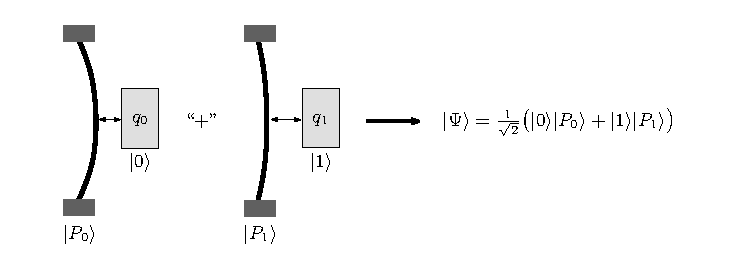
\includegraphics[width=.96\linewidth]{figures/ch06_fig27.pdf}
\caption{Armour、Blencowe、Schwab\cite{ref312}が提案した、ナノ機械共振器の二つの異なる位置の重ね合わせを生成する方法。箱の超伝導島の異なる電荷$q_0$、$q_1$に対応する基底状態$|0\rangle$、$|1\rangle$で記述されるCooper対箱を、共振器へ静電結合する。箱をコヒーレント重ね合わせ$(|0\rangle+|1\rangle)/\sqrt2$に準備し、適切な制御パルス列を加えると、もつれた箱・共振器の重ね合わせ$(|0\rangle|P_0\rangle+|1\rangle|P_1\rangle)/\sqrt2$が得られる。$|P_0\rangle$、$|P_1\rangle$は、共振器の識別できる二つの重心位置に対応する。}
\end{figure}

\subsubsectionlink*{QEMSにおけるデコヒーレンス}
上述の生成法の実用的な実現可能性を評価するには、その重ね合わせに影響するデコヒーレンスの主な源を理解することが重要である。まず、Cooper対箱自体も、もちろんデコヒーレンスを受ける。しかし、6.3.4節で述べたように、$\mu\mathrm s$領域の比較的長い時間は実験的に達成可能である\cite{ref289}。したがって、共振器自体の環境相互作用によるデコヒーレンスに焦点を当てられる。

興味深いことに、現在の実験的証拠\cite{ref318,ref319}、および初期の結果（たとえば\cite{ref320,ref321}）は、QEMSの主な散逸源、したがってデコヒーレンス源も、共振器の最低の基本曲げモードと、共振器内の局在した欠陥との相互作用かもしれないことを示す。これらの欠陥は有効二準位系で、電荷トラップ、不純物原子、弾性中心、共振器表面の結晶構造の乱れによる未結合手など、さまざまな物理的実現を取る。

現時点では、欠陥の基礎にある正確な物理的詳細や、曲げモードとの相互作用は、実験でも理論でも、まだ十分理解されていない。上述の空間的重ね合わせはまだ実現されていないため、QEMSのデコヒーレンスの直接実験データは存在しない。しかし、近年の実験は、散逸の特徴的性質について、貴重な情報を与えた\cite{ref318,ref319}。

散逸には一般にデコヒーレンスが伴うが、その逆は成り立たないので、こうした測定から、デコヒーレンスの性質についても知見を得られる。たとえば散逸データから、欠陥で構成される環境の有効スペクトル密度を取り出せるかもしれない。共振器と欠陥の相互作用の適切な模型があれば、それを使って、関係するデコヒーレンス係数と動力学を計算できる。そして、上述の重ね合わせの特徴的デコヒーレンス率を評価し、生成法の実現可能性を検討できる。ゆえに、QEMSの散逸とデコヒーレンスの現実的模型の開発が、主要な目標の一つとなる\cite{ref242,ref314,ref315}。それは理論的理解を高めるだけでなく、重ね合わせの実験的実現を前進させ、QEMSの実装全般の改善も示唆する。

% 原文 p.288
\hypertarget{srcpage:288}{}\label{srcpage:288}
Armour、Blencowe、Schwabは、最初の提案\cite{ref312}で、5.2節のよく研究された量子Brown運動模型を用い、空間的な箱・共振器重ね合わせ(6.37)のデコヒーレンス時間を評価した。中心調和振動子が基本曲げモードを表し、ほかの調和振動子からなる環境へ弱く結合する。しかし上述のように、mK温度のナノ機械共振器の環境は、欠陥を表す二準位系の集まりとして記述する方が、より現実的かもしれない。これらを量子スピン$1/2$粒子として模型化すれば、振動子・スピン模型が得られる。その弱結合マスター方程式は、5.4.2節で導いた［(5.198)参照］。

しかし、この模型の減衰率の温度依存性［(5.200)参照］は、散逸率が温度とともに増加するというQEMSの実験データ\cite{ref318,ref319}と一致しない。この不一致は、欠陥の少なくとも一部を、さらに別の、デコヒーレンスと散逸を生む環境に強く結合した、スピン$1/2$粒子として扱うべきことを示す（図6.28）。この環境は、スピンのトンネルを非コヒーレントにし、緩和も生じさせ、古典的二準位揺動子に似た欠陥動力学を誘起する。スピン浴から過剰エネルギーを吸収することで、その飽和を防ぐ。したがって、より現実的な模型は、独立なスピン・ボソン模型、すなわち振動子浴と相互作用するスピンを複数個、中心調和振動子へ結合したものかもしれない。この模型の最初の研究は、ごく最近行われた\cite{ref242}。このようにQEMSは、異なるデコヒーレンス・散逸模型を、実験で区別し検証する機会を与える。
\begin{figure}[htbp]\centering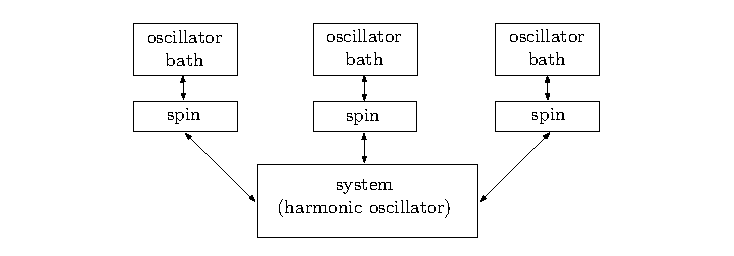
\includegraphics[width=.86\linewidth]{figures/ch06_fig28.pdf}
\caption{QEMSのデコヒーレンスと散逸の、考えられる模型。中心系は、ナノ機械共振器の基本曲げモードを表す調和振動子からなる。これは、スピン$1/2$粒子として模型化した二準位欠陥の集合と相互作用する。さらに各スピンは、散逸的な振動子浴へ結合し、その浴が、そうしなければ容易に飽和するスピン環境から、エネルギーを吸収する。}
\end{figure}

% 原文 p.289
\hypertarget{srcpage:289}{}\label{srcpage:289}
\subsectionlink{展望}
Schrödingerが1935年に猫の逆説を初めて描いたとき、それを純粋な思考実験、経験する巨視的世界へ量子力学を適用したときに生じる、明らかに「不合理な」帰結の例と考えた。しかし、過去数年、比較的小さいとはいえ、それでも巨視的なSchrödingerの猫を、実験室で育て、観測することに、大きな進展があった。本章では、数十個の光子を含む、巨視的に区別できる二状態の重ね合わせの生成（6.1節）、重い$\mathrm C_{70}$分子の干渉模様の観測（6.2節）、逆方向に流れる二つの$\mu\mathrm A$電流の重ね合わせの存在の検証（6.3節）を達成した実験を述べた。

各実験で研究者は、デコヒーレンスの漸進的作用、すなわち環境との相互作用により、重ね合わせがやがて観測できなくなる様子も、明示的に測定できた。こうして、量子から古典への移行の滑らかさを、明瞭に見た。量子状態を古典状態へ不連続に変換するような、固定された障壁は、量子領域と古典領域の間にない。系と環境の相互作用を操作することで、移行の動力学と時間尺度を直接変えられる。

したがって、本章の実験は、デコヒーレンスの範囲が、周囲の巨視的物体の、実効的に瞬時の「局在化」を指すだけよりも、はるかに広いことを示す。デコヒーレンスは、実効的古典性の出現を、漸進的で制御可能な過程として説明する。それは実験室で直接観測・検証でき、標準的量子力学の形式で厳密に理論記述できる。

ここでは、理論と実験の相互作用が非常に密接である。デコヒーレンス時間尺度や、その動力学のほかの性質の測定によって、模型を実験室で直接試せる。そして、模型がどの程度現実的で、物理的に適切かを学ぶ。一方、模型は、既存と将来の実験について貴重な情報を与える。ある配置で、どの段階の「巨視性」で量子から古典への移行を予想すべきか、あるパラメーターの組でどの種の「Schrödingerの子猫」を生成・観測できそうか、さらに「猫らしい」重ね合わせを作るため、実験をどう改善できるかを教える。本章では、理論的方式で提案された特定の重ね合わせの生成を、まだ達成していない二領域、Bose--Einstein凝縮（6.4.1節）と量子電気機械系（6.4.2節）を述べた。それでも、測定データとデコヒーレンス模型を組み合わせれば、望ましい重ね合わせを「見る」のを妨げる、物理的に関係する機構を同定でき、
% 原文 p.290
\hypertarget{srcpage:290}{}\label{srcpage:290}
有害な効果を弱める方法が示唆される。

自然に生じる問いは、巨視的に異なる状態の重ね合わせの実験が、将来どこへ向かうのか、その結果が量子力学の理解や、量子コンピューターなどの大規模量子系の構築に、どのような含意を持つか、ということである。答えは多いので、主要な点を少しだけ挙げよう。

まず、これまで調べた尺度では、既存の実験的証拠は、重ね合わせ原理の根本的限界を示していない。環境との望ましくない相互作用を最小にする適切な設計で、デコヒーレンスを十分制御できる限り、その限界は精密な定量解析が可能だが、「古典的」状態のどのような数の重ね合わせも、生成・観測できるように見える。

したがって、今後数年、巨視的に異なる状態の重ね合わせの、達成可能な「大きさ」の限界を、さらに押し進める多くの実験を見ることになる、といってよい。近いうちに、ウイルスのような、さらに大きい生体分子の干渉模様を観測し、凝縮体やナノ機械共振器の重ね合わせを実現し、超伝導量子ビットのデコヒーレンス時間を飛躍的に延ばせるかもしれない。このような実験は、重ね合わせ原理が破れる可能性を探し続けることによっても動機づけられる。しかし、デコヒーレンスは局所観測者からは見かけの破れを生じさせるので、十分にそれを遮蔽しながら、ユニタリー発展からのずれを誘起する機構には適度に敏感な実験を設計するのは、今後も非常に難しいだろう（8.4節および\cite{ref286,ref322}参照）。

ますます異なる巨視的状態の重ね合わせを生成・観測できることは、その重ね合わせ自体や、デコヒーレンスと量子力学一般に関わる、根本的な解釈上の問いを解かないことを、強調する必要がある。量子状態（2.1節）、特に重ね合わせ状態（2.2.1節）の適切な解釈と物理的意味の問題は、2.2.2節のStern--Gerlach実験のような、微視的設定ですでに明らかである。近年の巨視的重ね合わせ実験は、Schrödingerの猫型の直観に反する色合いを加えるかもしれないが、解釈の根本問題を解きも、深めもしない。

特に、環境を含む全体の量子状態でコヒーレンスが持続することをどう理解するか、したがって、デコヒーレンスの密度行列記述から生じる量子状態の非真正混合を、基礎にある何らかの量子的実在へどう適切に関係づけるかは、基礎論上の論争であり続ける。
% 原文 p.291
\hypertarget{srcpage:291}{}\label{srcpage:291}
ここで論じた型の実験は、少なくとも「実在の本性」についての先入観へ、さらに挑むことで、議論を今後も明るく照らすだろう。純粋にユニタリーな動力学からのずれを、実験が決定的に示す、あるいは排除できるようになれば、量子力学と量子的実在の構造について、新たな知見を得るか、得ざるを得なくなるかもしれない。しかし現在は、本章の驚くべき実験的成果を踏まえても、解釈の問題は残り続ける。


